\chapter{SCHR\"ODINGER'S EQUATION}
\section{Schr\"odinger's equation}\label{Schr\"odinger's equation}
The form of the wave equation of a physical sysytem is detemined by its Hamiltonian, which is therefore of fundamental significance in the whole mathematical fomulation of quantum mechanics.

The form of the Hamiltonian for a free particle is established by the general requirements imposed by the homogeneity and isotropy of space and by Galileo’s relativity principle. In classical mechanics, these requirements lead to a quadratic dependence of the energy of the particle on its momentum: $ E = p^2/2m $, where the constant $ m $ is called the mass of the particle (see Mechanics, §4). In quantum mechanics, the same requirements lead to a corresponding relation for the energy and momentum eigenvalues, these quantities being conserved and simultaneously measurable (for a free particle).

If the relation $ E = p^2/2m $ holds for every eigenvalue of the energy and momentum, the same relation must hold for their operators also:
\begin{equation}\label{17.1}
\hat{H}=\frac{1}{2m}\left(\hat{p}^2_x+\hat{p}^2_y+\hat{p}^2_z. \right)
\end{equation}
Substituting here from \eqref{15.2}, we obtain the Hamiltonian of a freely moving particle in the form
\begin{equation}\label{17.2}
\hat{H}=-\frac{\h}{2m}\Delta
\end{equation}
where $ \Delta=\p^2/{\p x}^2+\p^2/{\p y}^2+\p^2/{\p z}^2 $ is the Laplacian operator.

The Hamiltonian of a system of non-interacting particles is equal to the sum of the Hamiltonians of the separate particles:
\begin{equation}\label{17.3}
\hat{H}=-\frac{\h^2}{2}\sum_{a}\frac{\Delta_a}{m_a}
\end{equation}
(the suffix $ a $ is the number of the particle; $ \Delta_a $ is the Laplacian operator in which the differentiation is with respect to the coordinates of the $ a $th particle).

In classical (non-relativistic) mechanics, the interaction of particles is described by an additive term in the Hamiltonian, the potential energy of the interaction $ U(\bm{r}_1, \bm{r}_2,\dots) $, which is a function of the coordinates of the particles. By adding a similar function to the Hamiltonian of the system, the interaction of particles can be represented in quantum mechanics\footnote{This statement is, of course, not a logical consequence of the basic principles of quantum mechanics, and is to be regarded as a deduction from experiment.
}:
\begin{equation}\label{17.4}
\hat{H}=-\frac{\h^2}{2}\sum_{a}\frac{\Delta_a}{m_a}+U(\bm{r}_1, \bm{r}_2,\dots).
\end{equation}
The first term can be regarded as the operator of the kinetic energy and the second as that of the potential energy. In particular, the Hamiltonian for a single particle in an external field is
\begin{equation}\label{17.5}
\hat{H}=\frac{\hat{p}^2}{2m}+U(x,y,z)=-\frac{\h^2}{2m}\Delta+U(x,y,z),
\end{equation}
where $ U(x,y,z) $ is the potential energy of the particle in the external field.

Substituting the expressions \eqref{17.2} to \eqref{17.5} in the general equation \eqref{8.1}, we obtain the wave equations for the corresponding systems. We shall write out here the wave equation for a particle in an external field:
\begin{equation}\label{17.6}
\i\h\frac{\p \Psi}{\p t}=-\frac{\h^2}{2m}\Delta\Psi+U(x,y,z)
\end{equation}


The equation \eqref{10.2}, which determines the stationary states, takes the form
\begin{equation}\label{17.7}
\frac{\h^2}{2m}\Delta\psi+\left[ E-U(x,y,z)\right]\psi=0
\end{equation}
The equations \eqref{17.6} and \eqref{17.7} were obtained by Schr\"odinger in 1926 and are called \textit{Schr\"odinger's equations}.

For a free particle, equation \eqref{17.7} has the form
\begin{equation}\label{17.8}
\frac{\h^2}{2m}\Delta\psi+E\psi=0
\end{equation}


This equation has solutions finite in all space for any positive value of the energy $ E $. For states with definite directions of motion, these solutions are eigenfunctions of the momentum operator, with $ E = p^2/2m $. The complete (time-dependent) wave functions of such stationary states are
\begin{equation}\label{17.9}
\Psi=\text{const}\cdot\exp\left(\frac{\i}{\h}\left(Et-\bm{p}\bm{r}\right)\right).
\end{equation}


Each such function, a \textit{plane wave}, describes a state in which the particle has a definite energy $ E $ and momentum $ \bm{p} $. The angular frequency of this wave is $ E/\h $ and its wave vector $ \bm{k}=\bm{p}/\h $; the corresponding wavelength $ 2\pi\h/p $ is called the \textit{de Broglie wavelength} of the particle.\footnote{The idea of a wave related to a particle was first introduced by L. de Broglie in 1924.}

The energy spectrum of a freely moving particle is thus found to be continuous, extending from zero to $+\infty$. Each of these eigenvalues (except $ E = 0 $) is degenerate, and the degeneracy is infinite. For there corresponds to every value of $ E $, different from zero, an infinite number of eigenfunctions \eqref{17.9}, differing in the direction of the vector $ \bm{p} $, which has a constant absolute magnitude.

Let us enquire how the passage to the limit of classical mechanics occurs in Schrödinger’s equation, considering for simplicity only a single particle in an external field. Substituting in Schrödinger’s equation \eqref{17.6} the limiting expression \eqref{6.1} for the wave function,$ \Psi=ae^{\i S/\h} $ , we obtain, on performing the differentiation,
\[ a\frac{\p S}{\p t}-\i\h\frac{\p a}{\p t}+\frac{a}{2m}(\nabla S)^2-\frac{\i\h}{2m}a\Delta S-\frac{\i\h}{m}\nabla S\nabla a-\frac{\h^2}{2m}\Delta a+Ua=0. \]



In this equation there are purely real and purely imaginary terms (we recall that $ S $ and $ a $ are real); equating each separately to zero, we obtain two equations
\[ \frac{\p S}{\p t}+\frac{1}{2m}(\nabla S)^2+U-\frac{\h^2}{2ma}\Delta a=0, \]
\[ \frac{\p a}{\p t}+\frac{a}{2m}\Delta S+\frac{1}{m}\nabla S\nabla a=0. \]



Neglecting the term containing $\h$ in the first of these equations, we obtain
\begin{equation}\label{17.10}
\frac{\p S}{\p t}+\frac{1}{2m}(\nabla S)^2+U=0,
\end{equation}
that is; the classical Hamilton—Jacobi equation for the action $ S $ of a particle, as it should be. We see, incidentally, that, as $\h\rightarrow0  $ , classical mechanics is valid as far as quantities of the first (and not only the zero) order in ħ inclusive.

The second equation obtained above, on multiplication by $ 2a $, can be rewritten in the form
\begin{equation}\label{17.11}
\frac{\p a^2}{\p t}+\mathrm{div}\left( a^2\frac{\nabla S}{m}\right)=0
\end{equation}


This equation has an obvious physical meaning: $ a^2 $ is the probability density for finding the particle at some point in space($ \lvert\Psi\rvert^2=a^2 $);$ \nabla S/m=\bm{p}/m $ is the classical velocity $ \bm{v} $ of the particle. Hence equation \eqref{17.11} is simply the equation of continuity, which shows that the probability density “moves” according to the laws of classical mechanics with the classical velocity $ \bm{v} $ at every point.




{\small \textbf{PROBLEM}
	
	
Find the transformation law for the wave function in a Galilean transformation.





SOLUTION.Let us apply the transformation to the wave function for free motion of a particle (a plane wave). Since any function $\Psi$ can be expanded in plane waves, this will also give the transformation law for any wave function.

The plane waves in the frames of reference $ K $ and $ K' $ ($ K' $ moving with velocity $ V $ relative to $ K $) are
\[ \Psi(\bm{r},t)=\text{const}\cdot\exp\left[\i(\bm{p}\bm{r}-Et)/\h \right], \]
\[ \Psi'(\bm{r}',t)=\text{const}\cdot\exp\left[\i(\bm{p}'\bm{r}'-E't)/\h \right], \]
where $ \bm{r} = \bm{r}' + \bm{V}t $; the particle momenta and energies in the two frames are related by
\[ \bm{p}=\bm{p}'+m\bm{V},E=E'+\bm{V}\bm{p}'+mV^2/2 \]
(see Mechanics, \S8). Substitution of these expressions in $\Psi$ gives


\begin{multline}\label{(1)}
\Psi(\bm{r},t)=\Psi'(\bm{r}',t)\exp\left[\frac{\i}{\h}\left( m\bm{V}\bm{r}'+\frac{mV^2}{2}t\right)\right]=\notag\\
=\Psi'(\bm{r}-\bm{V}t,t)\exp\left[ \frac{\i}{\h}\left( m\bm{V}\bm{r}-\frac{mV^2}{2}t \right)\right].\tag{1}
\end{multline}
This formula does not contain the parameters of the free motion of the particle, and gives the required general transformation law for the wave function of any state of the particle. For a system of particles, the exponent in \eqref{(1)} contains a summation over the particles.
}
\section{The fundamental properties of Schr\"odinger's equation}\label{The fundamental properties of Schr\"odinger's equation}
The conditions which must be satisfied by solutions of Schrödinger’s equation are very general in character. First of all, the wave function must be single-valued and continuous in all space. The requirement of continuity is maintained even in cases where the field $ U(x, y, z) $ itself has a surface of discontinuity. At such a surface both the wave function and its derivatives must remain continuous. The continuity of the derivatives, however, does not hold if there is some surface beyond which the potential energy $ U $ becomes infinite. A particle cannot penetrate at all into a region of space where $ U=\infty $, i.e. we must have $ \psi = 0 $ everywhere in this region. The continuity of $\psi$ means that $\psi$ vanishes at the boundary of this region; the derivatives of $\psi$, however, in general are discontinuous in this case.

If the field $ U(x, y, z) $ nowhere becomes infinite, then the wave function also must be finite in all space. The same condition must hold in cases where $ U $ becomes infinite at some point but does so only as $ 1/r^s $ with $ s < 2 $ (see also \S35).

Let $ U_{\mathrm{min}} $ be the least value of the function $ U(x, y, z) $. Since the Hamiltonian of a particle is the sum of two terms, the operators of the kinetic energy $ \hat{T} $ and of the potential energy, the mean value $ \bar{E} $ of the energy in any state is equal to the sum $ \bar{T}+\bar{U} $. But all the eigenvalues of the operator $ \hat{T} $(which is the Hamiltonian of a free particle) are positive; hence the mean value $ \bar{T}\geqslant0 $. Recalling also the obvious inequality $ \bar{U}> U_{\mathrm{min}} $, we find that $ \bar{E}> U_{\mathrm{min}} $. Since this inequality holds for any state, it is clear that it is valid for all the eigenvalues of the energy:
\begin{equation}\label{18.1}
E_n>U_{\mathrm{min}}
\end{equation}
Let us consider a particle moving in an external field which vanishes at infinity; we define the function $ U(x, y, z) $, in the usual way, so that it vanishes at infinity. It is easy to see that the spectrum of negative eigenvalues of the energy will then be discrete, i.e. all states with $ E < 0 $ in a field which vanishes at infinity are bound states. For, in the stationary states of a continuous spectrum, which correspond to infinite motion, the particle reaches infinity (see \S\ref{Stationary states}); however, at sufficiently large distances the field may be neglected, the motion of the particle may be regarded as free, and the energy of a freely moving particle can only be positive.

The positive eigenvalues, on the other hand, form a continuous spectrum and correspond to an infinite motion; for $ E > 0 $, Schrödinger’s equation in general has no solutions (in the field concerned) for which the integral $ \int\lvert\psi\rvert^2\d V $ converges.\footnote{However, it must be mentioned that, for some particular mathematical forms of the function U (x, y, z) (which have no physical significance), a discrete set of values may be absent from the otherwise continuous spectrum.}

Attention must be drawn to the fact that, in quantum mechanics, a particle in a finite motion may be found in those regions of space where $ E < U $; the probability $ \lvert\psi\rvert^2 $ of finding the particle tends rapidly to zero as the distance into such a region increases, yet it differs from zero at all finite distances. Here there is a fundamental difference from classical mechanics, in which a particle cannot penetrate into a region where $ U>E $. In classical mechanics the impossibility of penetrating into this region is related to the fact that, for $ E < U $, the kinetic energy would be negative, that is, the velocity would be imaginary. In quantum mechanics, the eigenvalues of the kinetic energy are likewise positive; nevertheless, we do not reach a contradiction here, since, if by a process of measurement a particle is localized at some definite point of space, the state of the particle is changed, as a result of this process, in such a way that it ceases in general to have any definite kinetic energy.

If $ U(x, y, z)>0 $ in all space(and $ U\to0 $ at infinity), then, by the inequality \eqref{18.1}, we have $ E_n>0 $. Since, on the other hand, for E > 0 the spectrum must be continuous, we conclude that, in this case, the discrete spectrum is absent altogether, i.e. only an infinite motion of the particle is possible.

Let us suppose that, at some point (which we take as origin), $ U $ tends to $ -\infty $ in the manner
\begin{equation}\label{18.2}
U\approx-\alpha r^{-s},\quad\alpha>0.
\end{equation}
We consider a wave function finite in some small region (of radius $ r_0 $) about the origin, and equal to zero outside this region. The uncertainty in the values of the coordinates of a particle in such a wave packet is of the order of $ r_0 $; hence the uncertainty in the value of the momentum is $ \sim\h/r_0 $. The mean value of the kinetic energy in this state is of the order of $ \h^2/mr^2_0 $, and the mean value of the potential energy is $ \sim-\alpha/r^s_0 $. Let us first suppose that s < 2. Then the sum
\[ h^2/mr^2_0-\alpha/r^s_0 \]
takes arbitrarily larpe negative values for sufficiently small $ r_0 $. If, however, the mean energy can take such values, this always means that the energy has negative eigenvalues which are arbitrarily large in absolute value. The motion of the particle in a very small region of space near the origin corresponds to the energy levels with large $ \lvert E\rvert $. The “normal” state corresponds to a particle at the origin itself, i.e. the particle “falls” to the point $ r = 0 $.

If, however, s < 2, the energy cannot take arbitrarily large negative values. The discrete spectrum begins at some finite negative value. In this case the particle does not fall to the centre. It should be mentioned that, in classical mechanics, the fall of a particle to the centre would be possible in principle in any attractive field (i.e. for any positive $ s $). The case $ s = 2 $ will be specially considered in \S35.

Next, let us investigate how the nature of the energy spectrum depends on the behaviour of the field at large distances. We suppose that, as $ r\to\infty $, the potential energy, which is negative, tends to zero according to the power law \eqref{18.2} ($ r $ is now large in this formula), and consider a wave packet “filling” a spherical shell of large radius $ r_0 $ and thickness $ \Delta r\ll r_0 $. Then the order of magnitude of the kinetic energy is again $ \h^2/m(\Delta r)^2 $, and of the potential energy, $ -\alpha/r^s_0 $. We increase $ r_0 $, at the same time increasing $ \Delta r $, in such a way that $ \Delta r $ increases proportionally to $ r_0 $. If $ s < 2 $, then the sum becomes negative for sufficiently large $ r_0 $. Hence it follows that there are stationary states of negative energy, in which the particle may be found, with a fair probability, at large distances from the origin. This, however, means that there are levels of arbitrarily small negative energy (it must be recalled that the wave functions rapidly tend to zero in the region of space where $ U > E $). Thus, in this case, the discrete spectrum contains an infinite number of levels, which become denser and denser towards the level $ E = 0 $.

If the field diminishes as $ -1/r^s $ at infinity, with $ s>2 $, then there are not levels of arbitrarily small negative energy. The discrete spectrum terminates at a level with a non-zero absolute value, so that the total number of levels is finite.

Schr\"odinger's equation for the wave functions $\psi$ of stationary states is real, as are the conditions imposed on its solution. Hence its solutions can always be taken as real.\footnote{These assertions are not valid for systems in a magnetic field.} The eigenfunctions of non-degenerate values of the energy are automatically real, apart from the unimportant phase factor. For $\psi^*$ satisfies the same equation as $\psi$, and therefore must also be an eigenfunction for the same value of the energy; hence, if this value is not degenerate, $\psi$ and $\psi^*$ must be essentially the same, i.e. they can differ only by a constant factor (of modulus unity). The wave functions corresponding to the same degenerate energy level need not be real, however, but by a suitable choice of linear combinations of them we can always obtain a set of real functions.

The complete (time-dependent) wave functions $\Psi$ are determined by an equation in whose coefficients $ \i $ appears. This equation, however, retains the same form if we replace $ t $ in it by $ -t $ and at the same time take the complex conjugate.\footnote{It is assumed that the potential energy $ U $ does not depend explicitly on the time: the system is either closed or in a constant (non-magnetic) field.} Hence we can always choose the functions $\Psi$ in such a way that $\Psi$ and $\Psi^*$ differ only by the sign of the time.

As is well known, the equations of classical mechanics are unchanged by time reversal, i.e. when the sign of the time is reversed. In quantum mechanics, the symmetry with respect to the two directions of time is expressed, as we see, in the invariance of the wave equation when the sign of $ t $ is changed and $\Psi$ is simultaneously replaced by $\Psi^*$. However, it must be recalled that this symmetry here relates only to the equation, and not to the concept of measurement itself, which plays a fundamental part in quantum mechanics (as we have explained in detail in \S\ref{The wave function and measurements}).

\section{The current density}\label{The current density}
In classical mechanics the velocity $ \bm{v} $ of a particle is related to its momentum by $ \bm{p}=m\bm{v} $. A similar relation holds between the corresponding operators in quantum mechanics, as we should expect. This is easily shown by calculating the operator by the general rule \eqref{9.2} for the differentiation of operators with respect to time:
\[ \hat{\bm{v}}=\frac{\i}{\h}\left( \hat{H}\bm{r}-\bm{r}\hat{H}\right). \]
Using the expression \eqref{17.5} for $\hat{H}$ and formula \eqref{16.5}, we obtain
\begin{equation}\label{19.1}
\hat{\bm{v}}=\bm{p}/m
\end{equation}
Similar relations will clearly hold between the eigenvalues of the velocity and momentum, and between their mean values in any state.

The velocity, like the momentum of a particle, cannot have a definite value simultaneously with the coordinates. But the velocity multiplied by an infinitely short time interval $ \d t $ gives the displacement of the particle in the time $ \d t $. Hence the fact that the velocity cannot exist at the same time as the coordinates means that, if the particle is at a definite point in space at some instant, it has no definite position at an infinitely close subsequent instant.

We may notice a useful formula for the operator $ \hat{\dot{f}} $ of the derivative, with respect to time, of some quantity $ f(r) $ which is a function of the radius vector of the particle. Bearing in mind that $ f $ commutes with $ U(r) $, we find
\[ \hat{\dot{f}}=\frac{\i}{\h}\left(  \hat{H}f-f\hat{H} \right)=\frac{\i}{2m\h}\left( \hat{\bm{p}}^2f-f\hat{\bm{p}}^2\right). \]
Using \eqref{16.4}, we can write
\[ \hat{\bm{p}}^2f=\hat{\bm{p}}(f\hat{\bm{p}}-\i\h\nabla f),\quad f\hat{\bm{p}}^2=(\hat{\bm{p}}f-\i\h\nabla f)\hat{\bm{p}} \]
Thus we obtain the required expression:
\begin{equation}\label{19.2}
\hat{\dot{f}}=\frac{1}{2m}\left(\hat{\bm{p}}\nabla f+\nabla f\cdot\hat{\bm{p}} \right)
\end{equation}


Next, let us find the acceleration operator. We have
\[ \hat{\dot{\bm{v}}}=\frac{\i}{\h}\left(\hat{H}\hat{\bm{v}}-\hat{\bm{v}}\hat{H} \right)=\frac{\i}{m\h}\left( \hat{H}\hat{\bm{p}}-\hat{\bm{p}}\hat{H}\right)=\frac{\i}{m\h}\left( U\hat{\bm{p}}-\hat{\bm{p}}U\right) \]



Using formula \eqref{16.4}, we find
\begin{equation}\label{19.3}
m\hat{\dot{\bm{v}}}=-\nabla U.
\end{equation}
This operator equation is exactly the same in form as the equation of motion (Newton’s equation) in classical mechanics.

The integral $ \int\lvert\Psi\rvert^2\d V $, taken over some finite volume $ V $, is the probability of finding the particle in this volume. Let us calculate the derivative of this probability with respect to time. We have
\[ \frac{\d}{\d t}\int\lvert\Psi\rvert^2\d V=\int\left(\Psi\frac{\p\Psi^*}{\p t}+\Psi^*\frac{\p\Psi}{\p t} \right)\d V=\frac{\i}{\h}\int\left( \Psi\hat{H}^*\Psi^*-\Psi^*\hat{H}\Psi \right)\d V. \]
Substituting here
\[ \hat{H}=\hat{H}^*=-\frac{\h^2}{2m}\Delta+U(x,y,z) \]
and using the identity
\[ \Psi\Delta\Psi^*-\Psi^*\Delta\Psi=\mathrm{div}\left(\Psi\nabla\Psi^*-\Psi^*\nabla\Psi \right) \]
we obtain
\[ \frac{\d}{\d t}\int\lvert\Psi\rvert^2\d V=-\int\mathrm{div}\bm{j}\d V \]



where $ \bm{j} $ denotes the vector\footnote{If $\psi$ is written as $ \lvert\psi\rvert\e^{\i\alpha} $, then
	\begin{equation}\label{19.4a}
	\bm{j}=\frac{\h}{m}\lvert\psi\rvert^2\nabla\alpha\tag{19.4a}
	\end{equation}
}
\begin{equation}\label{19.4}
\bm{j}=\frac{\i\h}{2m}(\Psi\nabla\Psi^*-\Psi^*\nabla\Psi)=\frac{1}{2m}(\Psi\hat{\bm{p}}^*\Psi^*+\Psi^*\hat{\bm{p}}\Psi).
\end{equation}
The integral of $ \mathrm{div }\bm{j} $ can be transformed by Gauss’s theorem into an integral over the closed surface which bounds the volume V:
\begin{equation}\label{19.5}
\frac{\d}{\d t}\int\lvert\Psi\rvert^2\d V=-\oint\bm{j}\d\bm{f}
\end{equation}
It is seen from this that the vector $ \bm{j} $ may be called the \textit{probability current density} vector, or simply the \textit{current density}. The integral of this vector over a surface is the probability that the particle will cross the surface during unit time. The vector $ \bm{j} $ and the probability density $ \lvert\Psi\rvert^2 $ satisfy the equation
\begin{equation}\label{19.6}
\frac{\p\lvert\Psi\rvert^2}{\p t}+\mathrm{div}\bm{j}=0
\end{equation}
which is analogous to the classical equation of continuity.

The wave function of free motion (the plane wave \eqref{17.9}) can be normalized so as to describe a flow of particles with unit current density (in which, on average, one particle crosses a unit cross-section of the flow per unit time). This function is then
\begin{equation}\label{19.7}
\Psi=\frac{1}{\sqrt{v}}\exp\left[ -\frac{\i}{\h}(Et-\bm{p}\bm{r})\right],
\end{equation}
where $ v $ is the velocity of the particle, since substitution of this in \eqref{19.4} gives $ \bm{j}= \bm{p}/mv $, i.e. a unit vector in the direction of the motion.

It is useful to show how the orthogonality of the wave functions of states with different energies follows immediately from Schr\"odinger's equation. Let $\psi_m$ and $\psi_n$ be two such functions; they satisfy the equations
\begin{align*}
-\frac{\h^2}{2m}\Delta\psi_m+U\psi_m&=E_m\psi_m,\\
-\frac{\h^2}{2m}\Delta\psi_n^*+U\psi_n^*&=E_n\psi_n^*.
\end{align*}
We multiply the first of these by $ \psi_n^* $ and the second by $\psi_m$ and subtract corresponding terms; this gives
\[ (E_m-E_n)\psi_m\psi_n^*=\frac{\h^2}{2m}(\psi_m\Delta\psi_n^*-\psi_n^*\Delta\psi_m)=\frac{\h^2}{2m}\mathrm{div}(\psi_m\nabla\psi_n^*-\psi_n^*\nabla\psi_m). \]
If we now integrate both sides of this equation over all space, the right-hand side, on transformation by Gauss’s theorem, reduces to zero, and we obtain
\[ (E_m-E_n)\int\psi_m\psi_n^*\d V=0, \]
whence, by the hypothesis $ E_m\ne E_n $, there follows the required orthogonality relation
\[ \int\psi_m\psi_n^*\d V=0. \]
\section{The variational principle}\label{The variational principle}
Schr\"Odinger’s equation, in the general form $ \hat{H}\psi= E\psi $, can be obtained from, the variational principle
\begin{equation}\label{20.1}
\delta\int\psi^*(\hat{H}-E)\psi\d q=0
\end{equation}
Since $\psi$ is complex, we can vary $\psi$ and $\psi^*$ independently. Varying $\psi^*$, we have
\[ \int\delta\psi^*(\hat{H}-E)\psi\d q=0 \]
whence, because $ \delta\psi^* $ is arbitrary, we obtain the required equation $ \hat{H}\psi=E\psi $. The variation of $\psi$ gives nothing different. For, varying $\psi$ and using the fact that the operator $ \hat{H} $ is Hermitian, we have
\[ \int\psi^*(\hat{H}-E)\delta\psi\d q=\int\delta\psi(\hat{H}^*-E)\psi^*\d q=0 \]



from which we obtain the complex conjugate equation $ \hat{H}^*\psi^*=E\psi^* $.

The variational principle \eqref{20.1} requires an unconditional extremum of the integral. It can be stated in a different form by regarding $ E $ as a Lagrangian multiplier in a problem with the conditional extremum requirement
\begin{equation}\label{20.2}
\delta\int\psi^*\hat{H}\psi\d q=0
\end{equation}
the condition being
\begin{equation}\label{20.3}
\int\psi\psi^*\d q=1
\end{equation}

The least value of the integral in \eqref{20.2} (with the condition \eqref{20.3}) is the first eigenvalue of the energy, i.e. the energy $ E_0 $ of the normal state. The function $\psi$ which gives this minimum is accordingly the wave function $\psi_0$ of the normal state.\footnote{In the rest of this section we shall suppose the wave functions $\psi$ to be real; they can always be so chosen (if there is no magnetic field).} The wave functions $ \psi_n $($ n>0 $) of the other stationary states correspond only to an extremum, and not to a true minimum of the integral.

In order to obtain, from the condition that the integral in \eqref{20.2} is a minimum, the wave function $\psi_1$ and the energy $ E_1 $ of the state next to the normal one, we must restrict our choice to those functions $\psi$ which satisfy not only the normalization condition \eqref{20.3} but also the condition of orthogonality with the wave function $\psi_0$ of the normal state: $ \int\psi\psi_0\d q=0 $. In general, if the wave functions $ \psi_0,\psi_1,\dots,\psi_{n-1} $ of the first $ n $ states (arranged in order of increasing energy) are known, the wave function of the next state gives a minimum of the integral in \eqref{20.2} with the additional conditions
\begin{equation}\label{20.4}
\int\psi^2\d q=1,\quad\int\psi\psi_m\d q=0\quad m=0,1,2,\dots,n-1.
\end{equation}


We shall give here some general theorems which can be proved from the variational principle.\footnote{The proof of theorems concerning the zeros of eigenfunctions (see also \S\ref{General properties of motion in one dimension}) is given by M. A. Lavrent’ev and L. A. Lyusternik, \textit{The Calculus of Variations (Kurs variatsionnogo ischislemya)}, 2nd edition, chapter IX, Moscow, 1950; R. Courant and D. Hilbert, \textit{Methods of Mathematical Physics}, volume I, chapter VI, Interscience, New York, 1953.}

The wave function $\psi_0$ of the normal state does not become zero (or, as we say, has no \textit{nodes}) for any finite values of the coordinates.\footnote{This theorem and its consequences are not in general valid for the wave functions of systems consisting of several identical particles (see the end of \S63).} In other words, it has the same sign in all space. Hence, it follows that the wave functions $\psi_n$($ n>0 $) of the other stationary states, being orthogonal to $\psi_0$, must have nodes (if $\psi_n$ is also of constant sign, the integral $ \int\psi_0\psi_n\d q $ cannot vanish).

Next, from the fact that $\psi_0$ has no nodes, it follows that the normal energy level cannot be degenerate. For, suppose the contrary to be true, and let $\psi_0$, $\psi_0'$ be two different eigenfunctions corresponding to the level $ E_0 $. Any linear combination $ c\psi_0+c'\psi_0' $ will also be an eigenfunction; but by choosing the appropriate constants $ c $, $ c' $, we can always make this function vanish at any given point in space, i.e. we can obtain an eigenfunction with nodes.

If the motion takes place in a bounded region of space, we must have $ \psi=0 $ at the boundary of this region (see \S\ref{The fundamental properties of Schr\"odinger's equation}). To determine the energy levels, it is necessary to find, from the variational principle, the minimum value of the integral in \eqref{20.2} with this boundary condition. The theorem that the wave function of the normal state has no nodes means in this case that $\psi_0$ does not vanish anywhere inside this region.

We notice that, as the dimensions of the region containing the motion increase, all the energy levels $ E_n $ decrease; this follows immediately from the fact that an extension of the region increases the range of functions which can make the integral a minimum, and consequently the least value of the integral can only diminish.

The expression
\[ \int\psi\hat{H}\psi\d q=\int\left[-\sum_{a}\frac{\h^2}{2m_a}\psi\Delta_a\psi+U\psi^2  \right]\d q \]
for the states of the discrete spectrum of a particle system may be transformed into another expression which is more convenient in practice. In the first term of the integrand we write
\[ \psi\Delta_a\psi=\mathrm{div}_a(\psi\nabla_a\psi)-(\nabla_a\psi)^2. \]
The integral of $\mathrm{div}_a(\psi\nabla_a\psi)  $ over all space is transformed into an integral over an infinitely distant closed surface, and since the wave functions of the states of a discrete spectrum tend to zero sufficiently rapidly at infinity, this integral vanishes. Thus
\begin{equation}\label{20.5}
\int\psi\hat{H}\psi\d q=\int\left[\sum_{a}\frac{\h^2}{2m_a}(\nabla_a\psi)^2+U\psi^2  \right]\d q .
\end{equation}


\section{General properties of motion in one dimension}\label{General properties of motion in one dimension}
If the potential energy of a particle depends on only one coordinate ($ x $), then the wave function can be sought as the product of a function of $ y $ and $ z $ and a function of $ x $ only. The former of these is determined by Schr\"odinger's equation for free motion, and the second by the one-dimensional Schr\"odinger's equation
\begin{equation}\label{21.1}
\frac{\d^2\psi}{{\d x}^2}+\frac{2m}{\h^2}[E-U(x)]\psi=0
\end{equation}
Similar one-dimensional equations are evidently obtained for the problem of motion in a field whose potential energy is $ U (x, y, z) = U_1(x) + U_2(y) + U_3(z) $, i.e. can be written as a sum of functions each of which depends on only one of the coordinates. In \S\S\ref{The potential well}--\ref{Motion in a homogeneous field} we shall discuss a number of actual examples of such “one-dimensional” motion. Here we shall obtain some general properties of the motion.

We shall show first of all that, in a one-dimensional problem, none of the energy levels of a discrete spectrum is degenerate. To prove this, suppose the contrary to be true, and let $\psi_1$ and $\psi_2$ be two different eigenfunctions corresponding to the same value of the energy. Since both of these satisfy the same equation \eqref{21.1}, we have
\[ \frac{\psi_1''}{\psi_1}=\frac{2m}{\h^2}(U-E)=\frac{\psi_2''}{\psi_2} \]
or $ \psi_1''\psi_2-\psi_1\psi_2''=0 $ (the prime denotes differentiation with respect to $ x $). Integrating this relation, we find
\begin{equation}\label{21.2}
\psi_1'\psi_2-\psi_1\psi_2'=\mathrm{const}.
\end{equation}
Since $ \psi_1=\psi_2=0 $ at infinity, the constant must be zero, and so
\[\psi_1'\psi_2-\psi_1\psi_2'=0,  \]
or $ \psi_1'/\psi_1=\psi_2'/\psi_2 $. Integrating again, we obtain $ \psi_1=\mathrm{const}\cdot\psi_2 $, i.e. the two functions are essentially identical.

The following theorem (called the \textit{oscillation theorem}) may be stated for the wave functions $\psi_n(x)$ of a discrete spectrum. The function $\psi_n(x)$ corresponding to the ($ n + 1 $)th eigenvalue $ E_n $ (the eigenvalues being arranged in order of magnitude), vanishes $ n $ times (for finite\footnote{If the particle can be found only on a limited segment of the x-axis, we must consider the zeros of $\psi_n(x)$ within that segment.} values of $ x $).

We shall suppose that the function $ U (x) $ tends to finite limiting values as $ x \to \pm\infty $ (though it need not be a monotonic function). We take the limiting value $ U (+\infty) $ as the zero of energy (i.e. we put $ U (+\infty)=0 $), and we denote $ U (-\infty) $ by $ U_0 $, supposing that $ U_0>0 $. The discrete spectrum lies in the range of energy values for which the particle cannot move off to infinity; for this to be so, the energy must be less than both limiting values $ U (\pm\infty) $, i.e. it must be negative:
\begin{equation}\label{21.3}
E<0,
\end{equation}
and we must, of course, have in any case $ E > U_{\mathrm{min}} $, i.e. the function $ U (x) $ must have at least one minimum with $ U_{\mathrm{min}} < 0 $.

Let us now consider the range of positive energy values less than $ U_0 $:
\begin{equation}\label{21.4}
0<E<U_0
\end{equation}
In this range the spectrum will be continuous, and the motion of the particle in the corresponding stationary states will be infinite, the particle moving off towards $ x =+\infty $. It is easy to see that none of the eigenvalues of the energy in this part of the spectrum is degenerate either. To show this, it is sufficient to notice that the proof given above (for the discrete spectrum) still holds if the functions $\psi_1$, $\psi_2$ are zero at only one infinity (in the present case they tend to zero as $ x \to -\infty $).

For sufficiently large positive values of x, we can neglect $ U(x) $ in Schrödinger’s equation \eqref{21.1}:
\[ \psi''+\frac{2m}{\h^2}E\psi=0 \]



This equation has real solutions in the form of a stationary plane wave
\begin{equation}\label{21.5}
\psi=a\cos(kx+\delta)
\end{equation}
where $ a $ and $ \delta $ are constants, and the \textit{wave number}$ k=p/\h=\sqrt{2mE}/\h $. This formula determines the asymptotic form (for $ x\to+\infty $) of the wave functions of the non-degenerate energy levels in the range \eqref{21.4} of the continuous spectrum. For large negative values of $ x $, Schr\"odinger's equation is
\[ \psi''-\frac{2m}{\h^2}(U_0-E)\psi=0 \]
The solution which does not become infinite as $ x \to-\infty $ is
\begin{equation}\label{21.6}
\psi=b\e^{\varkappa x},\quad\varkappa=\frac{1}{2m}\sqrt{U_0-E}.
\end{equation}
This is the asymptotic form of the wave function as $ x\to\-\infty $. Thus the wave function decreases exponentially in the region where $ E < U $.

Finally, for
\begin{equation}\label{21.7}
E>U_0
\end{equation}
the spectrum will be continuous, and the motion will be infinite in both directions. In this part of the spectrum all the levels are doubly degenerate. This follows from the fact that the corresponding wave functions are determined by the second-order equation \eqref{21.1}, and both of the two independent solutions of this equation satisfy the necessary conditions at infinity (whereas, for instance, in the previous case one of the solutions became infinite as $ x\to-\infty $, and therefore had to be rejected). The asymptotic form of the wave function as $ x\to+\infty $ is
\begin{equation}\label{21.8}
\psi=a_1\e^{\i kx}+a_2\e^{-\i kx}
\end{equation}
and similarly for $ x\to-\infty $. The term $ \e^{\i kx} $ corresponds to a particle moving to the right, and $ \e^{-\i kx} $ corresponds to one moving to the left.

Let us suppose that the function $ U (x) $ is even [$ U (−x) = U (x) $]. Then Schr\"odinger's equation \eqref{21.1} is unchanged when the sign of the coordinate is reversed. It follows that, if $\psi(x)$ is some solution of this equation, then $\psi(-x)$ is also a solution, and coincides with $\psi(x)$ apart from a constant factor: $ \psi(-x)= c\psi(x) $. Changing the sign of $ x $ again, we obtain $ \psi(x)=c^2\psi(x) $, whence $ c = \pm1 $. Thus, for a potential energy which is symmetrical (relative to $ x = 0 $), the wave functions of the stationary states must be either even [$ \psi(-x)=\psi(x) $] or odd [$ \psi(-x)=-\psi(x) $].\footnote{In this discussion it is assumed that the stationary state is not degenerate, i.e. the motion is not infinite in both directions. Otherwise, when the sign of $ x $ is changed, two wave functions belonging to the energy level concerned may be transformed into each other. In this case, however, although the wave functions of the stationary states need not be even or odd, they can always be made so (by choosing appropriate linear combinations of the original functions).} In particular, the wave function of the ground state is even, since it cannot have a node, while an odd function always vanishes for $ x = 0 $ [$ \psi(0)=-\psi(0)=0 $].

To normalize the wave functions of one-dimensional motion (in a continuous spectrum), there is a simple method of determining the normalization coefficient directly from the asymptotic expression for the wave function for large values of $ \lvert x\rvert $.

Let us consider the wave function of a motion infinite in one direction, $ x \to+\infty$. The normalization integral diverges as $ x \to\infty $ (as $ x \to-\infty $, the function decreases exponentially, so that the integral rapidly converges). Hence, to determine the normalization constant, we can replace $\psi$ by its asymptotic value (for large positive $ x $), and perform the integration, taking as the lower limit any finite value of $ x $, say zero; this amounts to neglecting a finite quantity in comparison with an infinite one. We shall show that the wave function normalized by the condition
\begin{equation}\label{21.9}
\int\psi_p^*\psi_{p'}\d x=\delta\left(\frac{p-p'}{2\pi\h}\right)=2\pi\h\delta(p-p'), 
\end{equation}
where $ p $ is the momentum of the particle at infinity, must have the asymptotic form \eqref{21.5} with $ a = 2 $:
\begin{equation}\label{21.10}
\psi_p\approx2\cos(kx+\delta)=\e^{\i (kx+\delta)}+\e^{-\i(kx+\delta)}
\end{equation}
Since we do not intend to verify the orthogonality of the functions corresponding to different $ p $, on substituting the functions \eqref{21.10} in the normalization integral we shall suppose the momenta $ p $ and $ p' $ to be arbitrarily close; we can therefore put $ \delta=\delta' $ (in general $\delta$ is a function of $ p $). Next, we retain in the integrand only those terms which diverge for $ p = p' $; in other words, we omit terms containing the factor $ \e^{\pm\i (k+k')x} $. Thus we obtain
\[ \int\psi_p^*\psi_{p'}\d x=\int_{0}^{+\infty}\e^{\i(k'-k)x}\d x+\int_{0}^{+\infty}\e^{-\i(k'-k)x}\d x=\int_{-\infty}^{+\infty}\e^{\i(k'-k)x}\d x \]
which, from \eqref{15.7}, is the same as \eqref{21.9}.

The change to normalization by the delta function of energy is effected, in accordance with \eqref{5.14}, by multiplying $\psi_p$ by
\[ \left(\frac{\d(p/2\pi\h)}{\d E}\right)^{1/2}=\frac{1}{\sqrt{2\pi\h v}} \]
where $ v $ is the velocity of the particle at infinity. Thus
\begin{equation}\label{21.11}
\psi_E=\frac{1}{\sqrt{2\pi\h v}}\psi_p=\frac{1}{\sqrt{2\pi\h v}}(\e^{\i(kx+\delta)}+\e^{-\i(kx+\delta)})
\end{equation}
The current density is $ 1/(2\pi\h) $ in each of the travelling waves that make up the stationary wave \eqref{21.11}. Thus we can formulate the following rule for the normalization of the wave function for a motion infinite in one direction by the delta function of energy: having represented the asymptotic expression for the wave function in the form of a sum of two plane waves travelling in opposite directions, we must choose the normalization coefficient in such a way that the current density in the wave travelling towards (or away from) the origin is $ 1/(2\pi\h) $.

Similarly, we can obtain an analogous rule for normalizing the wave functions of a motion infinite in both directions. The wave function will be normalized by the delta function of energy if the sum of the probability currents in the waves travelling towards the origin from $ x =+\infty $ and $ x = -\infty $ is $ 1/(2\pi\h) $.
\section{The potential well}\label{The potential well}

As a simple example of one-dimensional motion, let us consider motion in a square potential well, i.e. in a field where $ U(x) $ has the form shown in FIG.\ref{Fig.1}:
\begin{wrapfigure}[11]{r}[0cm]{0cm}
	\begin{tikzpicture}
	\draw[->] (-2,0)--(3,0);
	\draw[->] (0,0)--(0,3);
	\draw[thick] (-1.5,1.5)--(0,1.5)--(0,0)--(1.5,0)--(1.5,1.5)--(3,1.5);
	\coordinate[label=right:$U_0$] (U0) at (0,1.5);
	\coordinate[label=below:$a$](a) at (1.5,0);
	\coordinate[label=left:$ U(x) $](Ux) at (0,3);
	\coordinate[label=below:$ x $](x) at (3,0);
	\end{tikzpicture}\caption{FIG.1}\label{Fig.1}
\end{wrapfigure}	
$ U (x) = 0 $ for $ 0 < x < a $, $ U (x) = U_0 $ for $ x < 0 $ and $ x > a $. It is evident a priori that for $ E < U_0 $ the spectrum will be discrete, while for $ E > U_0 $ we have a continuous spectrum of doubly degenerate levels.

In the region $ 0 < x < a $ we have Schr\"odinger's equation
\begin{equation}\label{22.1}
\psi''+\frac{2m}{\h^2}E\psi=0
\end{equation}
(the prime denotes differentiation with respect to $ x $), while in the region outside the well
\begin{equation}\label{22.2}
\psi''+\frac{2m}{\h^2}(E-U_0)\psi=0
\end{equation}
For $ x = 0 $ and $ x = a $ the solutions of these equations must be continuous together with their derivatives, while for $ x = \pm\infty $ the solution of equation \eqref{22.2} must remain finite (for the discrete spectrum when $ E < U_0 $, it must vanish).

For $ E < U_0 $, the solution of equation \eqref{22.2} which vanishes at infinity is $ \psi=\mathrm{const}\cdot\e^{\mp\varkappa x} $, where
\begin{equation}\label{22.3}
\varkappa=\frac{1}{\h}\sqrt{2m(U_0-E)};
\end{equation}
the signs $ - $ and $ + $ in the exponent refer to the regions $ x > a $ and $ x < 0 $ respectively. The probability $ |\psi|^2 $ of finding the particle decreases exponentially in the region where $ E < U (x) $. Instead of the continuity of $\psi$ and $\psi'$ at the edge of the potential well, it is convenient to require the continuity of $\psi$ and of its logarithmic derivative $\psi'/\psi$. Taking account of \eqref{22.3}, we obtain the boundary condition in the form
\begin{equation}\label{22.4}
|\psi'|/\psi=\mp\varkappa
\end{equation}
We shall not pause here to determine the energy levels in a well of arbitrary depth $ U_0 $ (see Problem 2), and shall analyse fully only the limiting case of infinitely high walls ($ U_0\to\infty $).

For $ U_0 = \infty $, the motion takes place only between the points $ x = 0 $ and $ x = a $ and, as was pointed out in \S\ref{The fundamental properties of Schr\"odinger's equation}, the boundary condition at these points is
\begin{equation}\label{22.5}
\psi=0
\end{equation}
(It is easy to see that this condition is also obtained from the general condition \eqref{22.4}. For, when $ U_0\to\infty $, we have also $ \varkappa\to\infty $ and hence $ \psi'/\psi\to\infty $; since $\psi'$ cannot become infinite, it follows that $ \psi= 0 $.) We seek a solution of equation \eqref{22.1} inside the well in the form
\begin{equation}\label{22.6}
\psi=c\sin(kx+\delta),\quad k=\frac{\sqrt{2mE}}{\h}.
\end{equation}
The condition $ \psi = 0 $ for $ x = 0 $ gives $ \delta = 0 $, and then the same condition for $ x = a $ gives $ \sin ka = 0 $, whence $ ka = n\pi $, $ n $ being a positive integer,\footnote{For $ n = 0 $ we should have $ \psi = 0 $ identically.} or
\begin{equation}\label{22.7}
E_n=\frac{\pi^2\h^2}{2ma^2}n^2,\quad n=1,2,3,\dots
\end{equation}
This determines the energy levels of a particle in a potential well. The normalized wave functions of the stationary states are
\begin{equation}\label{22.8}
\psi_n=\sqrt{\frac{2}{n}}\sin\left( \frac{\pi n}{a}x\right). 
\end{equation}


From these results we can immediately write down the energy levels for a particle in a rectangular “potential box”, i.e. for three-dimensional motion in a field whose potential energy $ U = 0 $ for $ 0 < x < a $, $ 0 < y < b $, $ 0 < z < c $ and $ U = \infty $ outside this region. In fact, these levels are given by the sums
\begin{equation}\label{22.9}
E_{n_1n_2n_3}=\frac{\pi^2\h^2}{2m}\left(\frac{n_1^2}{a^2}+\frac{n_2^2}{b^2}+\frac{n_3^2}{c^2} \right),\quad n_1,n_2,n_3=1,2,3,\dots,
\end{equation}
and the corresponding wave functions by the products
\begin{equation}\label{22.10}
\psi_{n_1n_2n_3}=\sqrt{\frac{8}{abc}}\sin\left(\frac{\pi n_1}{a}x \right)\sin\left(\frac{\pi n_2}{b}y \right)\sin\left(\frac{\pi n_3}{c}z \right).
\end{equation}


It may be noted that the energy $ E_0 $ of the ground state is, by \eqref{22.7} or \eqref{22.9}, of the order of $ \h^2/ml^2 $, where $ l $ is the linear dimension of the region in which the particle moves. This result is in accordance with the uncertainty relation; when the uncertainty in the coordinate is $ \sim l $, the uncertainty in the momentum, and therefore the order of magnitude of the momentum itself, is $\sim \h/l $. The corresponding energy is $\sim (\h/l)^2/m $.



{\small 

\textbf{PROBLEMS}


\textbf{1.} Determine the probability distribution for various values of the momentum for the normal state of a particle in an infinitely deep square potential well.





SOLUTION. The coefficients $ a (p) $ in the expansion of the function $\psi_1$ \eqref{22.8} in terms of the eigenfunctions of the momentum are
\[ a(p)=\int\psi_p^*\psi_1\d x=\sqrt{\frac{2}{a}}\int_0^a\sin\left(\frac{\pi}{a}x  \right)\exp\left(  -\i\frac{px}{\h}\right)\d x. \]
Calculating the integral and squaring its modulus, we obtain the required probability distribution:
\[ |a(p)|^2\frac{\d p}{2\pi\h}=\frac{4\pi\h^3a}{(p^2a^2-\pi^2\h^2)^2}\cos^2\frac{pa}{2\h}\d p. \]




\textbf{2.} Determine the energy levels for the potential well shown in FIG.\ref{Fig.2}.


SOLUTION. The spectrum of energy values $ E < U_1 $, which we shall consider, 
\begin{wrapfigure}[11]{l}[0cm]{0cm}
	\begin{tikzpicture}
	\draw[->] (-2,0)--(3,0);
	\draw[->] (0,0)--(0,3);
	\draw[thick] (-1.5,1)--(0,1)--(0,0)--(1.5,0)--(1.5,2)--(3,2);
	\coordinate[label=right:$U_1$] (U1) at (0,1);
	\coordinate[label=left:$U_2$](U2) at (1.5,2);
	\coordinate[label=below:$a$](a) at (1.5,0);
	\coordinate[label=left:$ U(x) $](Ux) at (0,3);
	\coordinate[label=below:$ x $](x) at (3,0);
	\end{tikzpicture}\caption{FIG.2}\label{Fig.2}
\end{wrapfigure}
is discrete. In the region $ x < 0 $ the wave function is
\[ \psi=c_1\e^{\varkappa_1 x},\quad \varkappa_1=(1/\h )\sqrt{2m(U_1-E)},\]
while in the region $ x > a $
\[ \psi=c_2\e^{-\varkappa_2 x},\quad \varkappa_2=(1/\h )\sqrt{2m(U_2-E)}. \]
Inside the well ($ 0 < x < a $) we look for $\psi$ in the form
\[ \psi=c\sin(kx+\delta),\quad k=\sqrt{2mE}/\h. \]
The condition of the continuity of $ \psi'/\psi $ at the edges of the well gives the equations
\[ k\cot\delta=\varkappa_1=\sqrt{\frac{2m}{\h^2}U_1-k^2},\quad k\cot(ka+\delta)=-\varkappa_2=-\sqrt{\frac{2m}{\h^2}U_2-k^2} ,\]
or
\[ \sin\delta=\frac{k\h}{\sqrt{2mU_1}},\quad \sin(ka+\delta)=-\frac{k\h}{\sqrt{2mU_2}} .\]
Eliminating $\delta$, we obtain the transcendental equation
\begin{equation}\label{3-(1)}
ka=n\pi-\arcsin\frac{k\h}{\sqrt{2mU_1}}-\arcsin\frac{k\h}{\sqrt{2mU_2}}\tag{1}
\end{equation}
(where $ n = 1, 2, 3,\dots, $ and the values of the inverse sine are taken between $ 0 $ and $ \pi/2 $), whose roots determine the energy levels $ E = k^2\h^2/2m $. For each $ n $ there is in general one root; the values of $ n $ number the levels in order of increasing energy.

Since the argument of the inverse sine cannot exceed unity, it is clear that the values of $ k $ can lie only in the range from $ 0 $ to $ \sqrt{2mU_1}/\h $. The left-hand side of equation \eqref{3-(1)} increases monotonically with $ k $, and the right-hand side decreases monotonically. Hence it is necessary, for a root of equation \eqref{3-(1)} to exist, that for the right-hand side should be less than the left-hand side. In particular, the inequality
\begin{equation}\label{3-(2)}
a\frac{\sqrt{2mU_1}}{\h}\geqslant\frac{\pi}{2}-\arcsin\sqrt{\frac{U_1}{U_2}},\tag{2}
\end{equation}
which is obtained for $ n = 1 $, is the condition that at least one energy level exists in the well. We tee that for given and unequal $ U_1 \ne U_2 $, there are always widths a of the well which are so small that there is no discrete energy level. For $ U_1 = U_2 $, the condition \eqref{3-(2)} is evidently always satisfied.

For $ U_1 = U_2 = U_0 $ (a symmetrical well), equation \eqref{3-(1)} reduces to
\begin{equation}\label{3-(3)}
\arcsin\frac{\h k}{\sqrt{2mU_0}}\frac{n\pi-ka}{2}.\tag{3}
\end{equation}
Introducing the variable $ \xi=ka/2 $, we obtain for odd $ n $ the equation
\begin{equation}\label{3-(4)}
\cos\xi=\pm\gamma\xi,\quad\gamma=\frac{\h}{a}\sqrt{\frac{2}{mU_0}},\tag{4}
\end{equation}
and those roots of this equation must be taken for which $ \tan \xi > 0 $. For even $ n $ we obtain the equation
\begin{equation}\label{3-(5)}
\sin\xi=\pm\gamma\xi,\tag{5}
\end{equation}
and we must take those roots for which $ \tan \xi < 0 $. The roots of these two equations determine the energy levels $ E=2\xi^2\h^2/ma^2 $. The number of levels is finite when $ \gamma\ne0 $.

In particular, for a shallow well in which $ U_0\ll \h^2/ma^2 $, we have $ \gamma\gg 1 $ and equation \eqref{3-(5)} has no root. Equation \eqref{3-(4)} has one root (with the upper sign on the right-hand side), $ \xi\approx(1/\gamma)(1-1/2\gamma^2) $. Thus the well contains only one energy level,
\[ E_0\approx U_0-\frac{ma^2}{2\h^2}U_0^2 \]
which is near the top of the well.





\textbf{3.} Determine the pressure exerted on the walls of a rectangular “potential box” by a particle inside it.





SOLUTION. The force on the the wall perpendicular to the $ x $-axis is the mean value of the derivative $ -\p H/\p a $ of the Hamilton’s function of the particle with respect to the length of the box in the direction of the $ x $-axis. The pressure is obtained by dividing this force by the area $ bc $ of the wall. According to the formula \eqref{11.16}, the required mean value is found by differentiating the eigenvalue \eqref{22.9} of the energy. The result is
\[ p^{(x)}=\frac{\pi^2\h^2}{ma^3bc}n_1^2. \]

}
\section{The linear oscillator}\label{The linear oscillator}
Let us consider a particle executing small oscillations in one dimension (what is called a \textit{linear oscillator}). The potential energy of such a particle is $ m\omega^2x^2/2 $, where $\omega$ is, in classical mechanics, the characteristic (angular) frequency of the oscillations. Accordingly, the Hamiltonian of the oscillator is
\begin{equation}\label{23.1}
\hat{H}=\frac{\hat{p}^2}{2m}+\frac{m\omega^2x^2}{2}.
\end{equation}


Since the potential energy becomes infinite for $ x = \pm\infty $, the particle can have only a finite motion, and the energy eigenvalue spectrum is entirely discrete.

Let us determine the energy levels of the oscillator, using the matrix method\footnote{This was done by Heisenberg in 1925, before Schr\"odinger's discovery of the wave equation.}. We shall start from the equations of motion in the form \eqref{19.3}; in this case they give
\begin{equation}\label{23.2}
\hat{\ddot{x}}+\omega^2x=0.
\end{equation}
In matrix form, this equation reads
\[ (\ddot{x})_{mn}+\omega^2x_{mn}=0. \]
For the matrix elements of the acceleration we have, according to \eqref{11.8}, $(\ddot{x})_{mn}=\i\omega_{mn}(\dot{x})_{mn}=-\omega_{mn}^2x_{mn}  $. Hence we obtain
\[ (\omega_{mn}^2-\omega^2)x_{mn}=0. \]
Hence it is evident that all the matrix elements $ x_{mn} $ vanish except those for which $ \omega_{mn}=\omega $ or $ \omega_{mn}=-\omega $. We number all the stationary states so that the frequencies $ \pm\omega $ correspond to transitions $ n\to n\mp 1$, i.e. $ \omega_{n,n\mp1}=\pm\omega $. Then the only non-zero matrix elements are $ x_{n,n\pm1} $.

We shall suppose that the wave functions $\psi_n$ are taken real. Since $ x $ is a real quantity, all the matrix elements $ x_{mn} $ are real. The Hermitian condition \eqref{11.10} now shows that the matrix $ x_{mn} $ is symmetrical:
\[ x_{mn}=x_{nm}. \]



To calculate the matrix elements of the coordinate which are different from zero, we use the commutation rule
\[ \hat{\dot{x}}\hat{x}-\hat{x}\hat{\dot{x}}=-\i\frac{\h}{m}, \]
written in the matrix form
\[ (\dot{x}x)_{mn}-(x\dot{x})_{mn}=-\frac{\i\h}{m}\delta_{mn} \]
By the matrix multiplication rule \eqref{11.12} we hence have for $ m = n $
\[ \i\sum_l(\omega_{nl}x_{nl}x_{ln}-x_{nl}\omega_{ln}x_{ln}) =2\i\sum_l\omega_{nl}x_{nl}^2=-\i\frac{\h}{m}.\]



In this sum, only the terms with $ l = n \pm 1 $ are different from zero, so that we have
\begin{equation}\label{23.3}
\left(x_{n+1,n}\right)^2-\left(x_{n,n-1}\right)^2=\frac{\h}{2m\omega}.
\end{equation}


From this equation we deduce that the quantities $  \left(x_{n+1,n}\right)^2$ form an arithmetic progression, which is unbounded above, but is certainly bounded below, since it can contain only positive terms. Since we have as yet fixed only the relative positions of the numbers $ n $ of the states, but not their absolute values, we can arbitrarily choose the value of $ n $ corresponding to the first (normal) state of the oscillator, and put this value equal to zero. Accordingly $ x_{0,−1} $ must be regarded as being zero identically, and the application of equations \eqref{23.3} with $ n = 0, 1,\cdots $ successively leads to the result
\[ \left(x_{n,n-1}\right)^2=\frac{n\h}{2m\omega} .\]



Thus we finally obtain the following expression for the matrix elements of the coordinate which are different from zero:\footnote{We choose the indeterminate phases $\alpha_n$ (see the second footnote to \S\ref{Matrices}) so as to obtain the plus sign in front of the radical in all the matrix elements \eqref{23.4}. Such a choice is always possible for a matrix in which only those elements are different from zero which correspond to transitions between states with adjacent numbers.
}
\begin{equation}\label{23.4}
x_{n,n-1}=x_{n-1,n}=\sqrt{\frac{n\h}{2m\omega}}
\end{equation}


The matrix of the operator $\hat{H}$ is diagonal, and the matrix elements $ H_{nn} $ are the required eigenvalues $ E_n $ of the energy of the oscillator. To calculate them, we write
\begin{multline*}
H_{nn}=E_n=\frac{m}{2}\left[ \left(\dot{x}^2\right)_{nn}+\omega^2(x^2)_{nn}\right]=\\
=\frac{m}{2}\left[\sum_l\i\omega_{nl}x_{nl}\i\omega_{ln}x_{ln}+\omega^2\sum_lx_{nl}x_{ln}  \right]=\frac{m}{2}\left(\omega^2+\omega_{nl}^2\right)x_{ln}^2.
\end{multline*}
In the sum over $ l $, only the terms with $ l = n\pm1 $ are different from zero; substituting \eqref{23.4}, we obtain
\begin{equation}\label{23.5}
E_n=(n+1/2)\h\omega,\quad n=0,1,2,\dots
\end{equation}


Thus the energy levels of the oscillator lie at equal intervals of $ \h\omega $ from one another. The energy of the normal state ($ n = 0 $) is $ \h\omega/2 $; we call attention to the fact that it is not zero.

The result \eqref{23.5} can also be obtained by solving Schr\"odinger's equation. For an oscillator, this has the form
\begin{equation}\label{23.6}
\frac{\d^2\psi}{{\d x}^2}+\frac{2m}{\h^2}\left( E-\frac{m\omega^2x^2}{2}\right)\psi=0
\end{equation}
Here it is convenient to introduce, instead of the coordinate $ x $, the dimensionless variable $\xi$ by the relation
\begin{equation}\label{23.7}
\xi=\sqrt{\frac{m\omega}{\h}}x.
\end{equation}
Then we have the equation
\begin{equation}\label{23.8}
\psi''+\left(\frac{2E}{\h\omega}-\xi^2 \right)\psi=0;
\end{equation}
here the prime denotes differentiation with respect to $\xi$.

For large $\xi$, we can neglect $ 2E/\h\omega $ in comparison with $\xi^2$; the equation $ \psi''= \xi^2\psi $ has the asymptotic integrals $ \psi=\e^{\pm\xi^2/2} $(for differentiation of this function gives $ \psi''= \xi^2\psi $ on neglecting terms of order less than that of the term retained). Since the wave function $\psi$ must remain finite as $\xi\to\pm\infty$, the index must be taken with the minus sign. It is therefore natural to make in equation \eqref{23.8} the substitution
\begin{equation}\label{23.9}
\psi=\e^{-\xi^2/2}\chi(\xi).
\end{equation}
For the function we obtain the equation (with the notation $ 2E/ħω −1 = 2n $; since we already know that $ E > 0 $, we have $ n > -1/2 $)
\begin{equation}\label{23.10}
\chi''-2\xi\chi'+2n\chi=0,
\end{equation}
where the function must be finite for all finite $\xi$, and for $\xi\to\pm\infty$ must not tend to infinity more rapidly than every finite power of $\xi$ (in order that the function $\psi$ should tend to zero).

Such solutions of equation \eqref{23.10} exist only for positive integral (and zero) values of $ n $ (see \S a of the Mathematical Appendices); this gives the eigenvalues \eqref{23.5} for the energy, which we know already. The solutions of equation \eqref{23.10} corresponding to various integral values of $ n $ are 
\[ \chi=\mathrm{const}\cdot H_n(\xi) ,\] 
where $ H_n(\xi) $ are what are called \textit{Hermite polynomials}; these are polynomials of the $ n $th degree in $\xi$, defined by the formula
\begin{equation}\label{23.11}
H_n(\xi)=(-1)^n\e^{\xi^2}\frac{\d^n \e^{-\xi^2}}{{\d \xi}^n}
\end{equation}
Determining the constants so that the functions $\psi_n$ satisfy the normalization condition
\[ \int_{-\infty}^{+\infty}\psi^2_n(x)\d x=1 \]
we obtain (see (a.7))
\begin{equation}\label{23.12}
\psi_n(x)=\left(\frac{m\omega}{\pi\h} \right)^{1/4}\frac{1}{\sqrt{2^n n!}}\exp\left(-\frac{m\omega}{2\h}x^2\right)H_n\left( x\sqrt{\frac{m\omega}{\h}}\right).
\end{equation}
Thus the wave function of the normal state is
\begin{equation}\label{23.13}
\psi_0(x)=\left(\frac{m\omega}{\pi\h} \right)^{1/4}\exp\left(-\frac{m\omega}{2\h}x^2\right).
\end{equation}
It has no zeros for finite $ x $, which is as it should be.

By calculating the integrals $ \int_{-\infty}^{+\infty}\psi_n\psi_m\xi\d \xi $, we can determine the matrix elements of the coordinate; this calculation leads, of course, to the same values \eqref{23.4}.

Finally, we shall show how the wave functions $\psi_n$ may be calculated by the matrix method. We notice that, in the matrices of the operators $ \hat{\dot{x}}\pm\i\omega\hat{x} $, the only elements different from zero are
\begin{equation}\label{23.14}
(\dot{x}-\i\omega x)_{n,n-1}=-(\dot{x}+\i\omega)_{n,n-1}-\i\sqrt{\frac{2\omega\h n}{m}}
\end{equation}



Using the general formula \eqref{11.11}, and taking into account the fact that $ ψ_{−1}\equiv 0 $, we conclude that
\[ \frac{\d \psi_0}{\d x}=-\frac{m\omega}{\h}x\psi_0, \]



After substituting the expression $ \hat{\dot{x}}=-\i\frac{\h}{m}\frac{\d}{\d x} $, we obtain the equation
\[ \frac{\d \psi_0}{\d x}=-\frac{m\omega}{\h}x\psi_0 \]
whose normalized solution is \eqref{23.13}. And, since
\[ (\hat{\dot{x}}+\i\omega\hat{x})\psi_{n-1}=(\dot{x}+\i\omega x)_{n,n-1}\psi_n=\i\sqrt{\frac{2\omega\h n}{m}}\psi_n, \]
we obtain the recurrence formula
\begin{multline*}
\psi_n=\sqrt{\frac{m}{2\omega\h n}}\left(-\frac{\h}{m}\frac{\d}{\d x}+\omega x \right)\psi_{n-1}=\frac{1}{\sqrt{2n}}\left(-\frac{\d}{\d\xi}+\xi \right)\psi_{n-1}=\\
=-\frac{1}{\sqrt{2n}}\exp\frac{\xi^2}{2}\frac{\d}{\d\xi}\left(\exp\left(-\frac{\xi^2}{2} \right)\psi_{n-1} \right),
\end{multline*}
when this is applied $ n $ times to the function \eqref{23.13}, we obtain the expression \eqref{23.12} for the normalized functions $\psi_n$.





{\small
\textbf{PROBLEMS}


\textbf{1.} Determine the probability distribution of the various values of the momentum for an oscillator.





SOLUTION. Instead of expanding the wave function of the stationary state in terms of the eigenfunctions of momentum, it is simpler in the case of the oscillator to start directly from Schr\"odinger's equation in the momentum representation. Substituting in \eqref{23.1} the coordinate operator \eqref{15.12}, we obtain the Hamiltonian in the $ p $ representation,
\[ \hat{H}=\frac{p^2}{2m}-\frac{m\omega^2\h}{2}\frac{\d^2}{{\d p}^2}. \]
The corresponding Schr\"odinger's equation$  \hat{H}a (p) = Ea (p) $ for the wave function $ a (p) $ in the momentum representation is
\[ \frac{\d^2 a(p)}{{\d p}^2}+\frac{2}{m\omega^2\h^2}\left( E-\frac{p^2}{2m}\right)a(p)=0. \]
This equation is of exactly the same form as \eqref{23.6}; hence its solutions can be written down at once by analogy with \eqref{23.12}. Thus we find the required probability distribution to be
\[ |a(p)|^2\frac{\d p}{2\pi\h}=\frac{1}{2^nn!\sqrt{\pi m\omega\h}}\exp\left(-\frac{p^2}{m\omega\h} \right)H_n^2\left( \frac{p}{\sqrt{m\omega\h}}\right) .\]




\textbf{2.} Determine the lower limit of the possible values of the energy of an oscillator, using the uncertainty relation \eqref{16.7}.





SOLUTION. Since $ \bar{x^2}=\bar{x}^2+(\delta x)^2 ,\bar{p^2}=\bar{p}^2+(\delta p)^2$, \eqref{16.7} gives for the mean value of the energy of the oscillator
\[ \bar{E}=\frac{m\omega^2}{2}\bar{x^2}+\frac{\bar{p^2}}{2m}\geqslant\frac{m\omega^2}{2}\bar{(\delta x)^2}+\frac{\bar{(\delta p)^2}}{2m}\geqslant\frac{m\omega^2\h^2}{8(\delta p)^2}+\frac{(\delta p)^2}{2m}. \]
On determining the minimum value of this expression (regarded as a function of $\delta p$), we find the lower limit of the mean values of the energy, and therefore that of all possible values: $ E\geqslant\h\omega/2. $




\textbf{3.} Find the wave functions of the states of a linear oscillator that minimize the uncertainty relation, i.e. in which the standard deviations of the coordinate and momentum in the wave packet are related by $  \delta p \delta x = \h/2 $ (E. Schr\"odinger 1926).\footnote{These are called \textit{coherent states}.}





SOLUTION. The required wave functions must have the form
\begin{equation}\label{23-1}
\Psi(x,t)=\frac{1}{(2\pi)^{1/4}(\delta x)^{1/2}}\exp\left\{\i\frac{\bar{p}x}{\h}-\frac{(x-\bar{x})^2}{4(\delta x)^2}-\i\phi(t)   \right\}.\tag{1}
\end{equation}
Their dependence on the coordinate at any instant is in accordance with \eqref{16.8}, $ \bar{x}=\bar{x}(t) $and $ \bar{p}=\bar{p}(t)=m\dot{\bar{x}}(t)$  being the mean values of the coordinate and the momentum; according to \eqref{19.3}, we have, for a linear oscillator ($ U = m\omega^2x^2/2 $), $ \hat{\dot{p}}=-m\omega^2x $, and therefore for the mean value $ \dot{\bar{p}}=-m\omega^2\bar{x} $ or
\begin{equation}\label{23-2}
\ddot{\bar{x}}+\omega^2\bar{x}=0\tag{2}
\end{equation}
i.e. the function satisfies the classical equation of motion. The constant factor in \eqref{23-1} is determined by the normalization condition $ \int_{-\infty}^{+\infty}|\Psi|^2\d x=1 $ in addition to this factor, $\Psi$ may contain a phase factor with a time-dependent phase $\phi(t)$. The unknown constant $\delta x$ and the unknown function $\phi(t)$ are found by substituting \eqref{23-1} in the wave equation
\[ -\frac{\h^2}{2m}\frac{\p^2\Psi}{{\p x}^2}+\frac{m\omega^2x^2}{2}\Psi=\i\h\frac{\p\Psi}{\p t} .\]
With \eqref{23-2}, the substitution gives
\[ \left(\frac{x^2}{2}-x\bar{x} \right)\left(\frac{m^2\omega^2}{\h^2}-\frac{1}{4(\delta x)^4} \right)+\left[\frac{m^2\dot{\bar{x}}^2}{2\h^2}-\frac{\bar{x}^2}{8(\delta x)^4}+\frac{1}{4(\delta x)^2}-\frac{m}{\h}\dot{\phi(t)} \right]=0 .\]
Hence $ (\delta x)^2 = \h/(2mω) $ and
\[ \dot{\phi}=\frac{m}{2\h}(\dot{\bar{x}}^2-\omega^2\bar{x}^2)+\frac{\omega}{2},\quad\phi=\frac{1}{2\h}\bar{p}\bar{x}+\frac{\omega}{2}t. \]
Thus we have finally
\begin{equation}\label{23-3}
\Psi(x,t)=\left(\frac{m\omega}{\pi\h} \right)^{1/4}\exp\left\{  \frac{\i\bar{p}x}{\h}-\frac{m\omega(x-\bar{x})^2}{2\h} \right\}\exp\left\{-\frac{\i\omega t}{2}-\frac{\i\bar{p}\bar{x}}{2\h} \right\}\tag{3}
\end{equation}


When $ \bar{x}=0 $ and $ \bar{p}=0 $, this becomes $ \psi_0(x)\e^{−\i\omega t/2} $, the wave function of the oscillator ground state.

The mean energy of the oscillator in a coherent state is
\begin{equation}\label{23-4}
\bar{E}=\frac{\bar{p^2}}{2m}+\frac{m\omega^2\bar{x^2}}{2}=\frac{\bar{p^2}}{2m}+\frac{m\omega^2\bar{x}^2}{2}+\frac{\h\omega}{2}\equiv\h\omega\left(\bar{n}+\frac{1}{2} \right);\tag{4}
\end{equation}
the quantity $\bar{n} $ is the mean “number” of quanta $ \h\omega $ in the state. We see that the coherent state is completely specified by the function $ \bar{x}(t) $ satisfying the classical equation \eqref{23-2}. The general form of this function may be given as
\begin{equation}\label{23-5}
\frac{m\omega\bar{x}+\i\bar{p}}{\sqrt{2m\h\omega}}a\e^{\i\omega t},\quad|a|^2=\bar{n}.\tag{5}
\end{equation}


The function \eqref{23-3} can be expanded in wave functions of the stationary states of the oscillator:
\[ \Psi=\sum_{n=0}^{\infty}a_n\Psi_n,\quad\Psi_n(x,t)=\psi_n(x)\exp\left\{-\i\left(n+\frac{1}{2} \right)\omega t \right\}. \]
The coefficients in this expansion are (cf. \S41, Problem 1)
\begin{equation}\label{23-6}
a_n=\int_{-\infty}^{+\infty}\Psi_n^*\Psi\d x.\tag{6}
\end{equation}
The probability for the oscillator to be in the $ n $th state is therefore
\begin{equation}\label{23-7}
\omega_n=|a_n|^2=\e^{-\bar{n}}\frac{\bar{n}^n}{n!}\tag{7}
\end{equation}
the Poisson distribution.





\textbf{4.} Determine the energy levels for a particle moving in a field of potential energy (Fig. \ref{Fig.3}; P. M. Morse)
\[ U(x)=A\left(\e^{-2\alpha x}-2\e^{-\alpha x} \right) .\]






SOLUTION. The spectrum of positive eigenvalues of the energy is continuous (and the levels are not degenerate), while the spectrum of negative eigenvalues is discrete.

Schr\"odinger's equation reads
\[ \frac{\d^2 \psi}{{\d x}^2}+\frac{2m}{\h^2}\left(E-A\e^{-2\alpha x}+2A\e^{-\alpha x} \right)\psi=0. \]
We introduce a new variable
\[ \xi=\frac{2\sqrt{2mA}}{\alpha\h}\e^{-\alpha x} \]
(taking values from $ 0 $ to $\infty$) and the notation (we consider the discrete spectrum, so that $ E < 0 $)
\begin{equation}\label{23-8}
s=\frac{\sqrt{-2mE}}{\alpha\h},\quad n=\frac{\sqrt{2mA}}{\alpha\h}+\left(s+\frac{1}{2}\right)\tag{1}
\end{equation}
Schr\"odinger's equation then takes the form
\[ \psi''+\frac{1}{\xi}\psi'+\left(-\frac{1}{4}+\frac{n+s+1/2}{\xi}-\frac{s^2}{\xi^2} \right)\psi=0 \]
As $ \xi\to\infty  $, the function $\psi$ behaves asymptotically as $ e^{\pm\xi/2} $, while as $ \xi\to0  $ it is proportional to $ \xi\pm s $. From considerations of finiteness we must choose the solution
\begin{wrapfigure}[13]{l}[0cm]{0cm}
	\begin{tikzpicture}
	\draw[->] (-2,0)--(4,0);
	\draw[->] (0,-2)--(0,2);
	\draw[ thick,domain =-0.87:3.5] plot(\x,{1.5*( exp(-2*\x)-2*exp(-1*\x))}); 
	\coordinate[label=right:$ U(x) $](Ux) at (0,2);
	\coordinate[label=below:$ x $](x) at (4,0);
	\coordinate[label=below left:$ -A $](-A) at (0,-1.5);
	\end{tikzpicture}\caption{FIG. 3}\label{Fig.3}
\end{wrapfigure}
which behaves as $ e^{-\xi/2} $ as $ \xi\to\infty $ and as $ \xi^s $ as $ \xi\to0  $. We make the substitution
\[ \psi=\e^{-\xi/2}\xi^s\omega(\xi) \]
and obtain for $\omega$ the equation
\begin{equation}\label{23-9}
\xi\omega''+(2s+1-\xi)\omega'+n\omega=0,\tag{2}
\end{equation}
which has to be solved with the conditions that $\omega$ is finite as $\xi\to0$, while as $\xi\to\infty$, $\omega$ tends to infinity not more rapidly than every finite power of $\xi$. Equation \eqref{23-9} is the equation for a confluent hypergeometric function (see \S d of the Mathematical Appendices):
\[ \omega=F(-n,2s+1,\xi). \]
A solution satisfying the required conditions is obtained for non-negative integral $ n $ (when the function $ F $ reduces to a polynomial). According to the definitions \eqref{23-8}, we thus obtain for the energy levels the values
\[ -E_n=\left[1-\frac{\alpha\h}{\sqrt{2mA}}\left(n+\frac{1}{2} \right) \right]^2. \]
where $ n $ takes positive integral values from zero to the greatest value for which (so that the parameter $ s $ is positive in accordance with its definition). Thus the discrete spectrum contains only a limited number of levels. If 
\[ \frac{\sqrt{2mA}}{\alpha\h}<\frac{1}{2}, \]
there is no discrete spectrum at all.





\textbf{5.} The same as Problem 4, but with $ U = -{\displaystyle \frac{U_0}{\cosh^2\alpha x}}$ (Fig. \ref{Fig.4}).
\vspace{1.2ex}





SOLUTION. The spectrum of positive eigenvalues of the energy is continuous, while that of negative values is discrete; we shall consider the latter. Schrödinger’s equation is
\[ \frac{\d^2\psi}{{\d x}^2}+\frac{2m}{\h}\left(E+\frac{U_0}{\cosh^2\alpha x} \right)\psi=0. \]
We put $ \xi= \tanh \alpha x $ and use the notation
\[ \epsilon=\frac{\sqrt{-2mE}}{\h\alpha},\quad\frac{2mU_0}{\alpha^2\h^2}=s(s+1),\quad s=\frac{1}{2}\left( -1+\sqrt{1+\frac{8mU_0}{\alpha^2\h^2}}\right), \]
obtaining
\begin{wrapfigure}[]{r}[0cm]{0cm}
	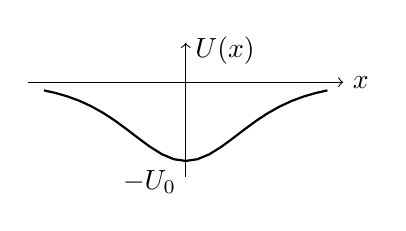
\begin{tikzpicture}
	\draw[->] (-2,0)--(2,0);
	\draw[->] (0,-1.2)--(0,0.5);
	\draw[ thick,domain =-1.8:1.8] plot(\x,{-1/( cosh(\x)*cosh(\x))}); 
	\coordinate[label=right:$ U(x) $](Ux) at (0,0.4);
	\coordinate[label=right:$ x $](x) at (2,0);
	\coordinate[label=below left:$ -U_0 $](-U0) at (0,-1);
	\end{tikzpicture}\caption{FIG. 4}\label{Fig.4}
\end{wrapfigure}
\[ \frac{\d}{\d\xi}\left[(1-\xi^2)\frac{\d\psi}{\d\xi} \right]+\left[s(s+1)-\frac{\epsilon^2}{1-\xi^2} \right]\psi=0. \]
This is the equation of the associated Legendre polynomials; it can be brought to hypergeometric form by making the substitution  
\[ \psi = (1 − \xi^2)^{\epsilon/2}w(\xi) \]  
and temporarily changing the variable to $ \frac{1}{2}(1 − ξ)=u $:
\[ u(1-u)w''+(\epsilon+1)(1-2u)w'-(\epsilon-s)(\epsilon+s+1)w=0. \]
The solution finite for $ \xi= 1 $ (i.e. for $ x = \infty $) is
\[ \psi=(1 − \xi^2)^{\epsilon/2}w(\xi)F[\epsilon-s,\epsilon+s+1,\epsilon-1,(1-\xi)/2]. \]
If $\psi$ remains finite for $ \xi= −1 $ (i.e. for $ x = -\inf $), we must have $\epsilon-s=-n$ where $ n = 0, 1, 2, \dots $; then $ F $ is a polynomial of degree $ n $, which is finite for $ \xi = −1 $. 

Thus the energy levels are determined by $\epsilon-s=-n$, or
\[ E_n=-\frac{\h^2\alpha^2}{8m}\left[ -(2n+1)+\sqrt{1+\frac{8mU_0}{\alpha^2\h^2}} \right]^2. \]
There is a finite number of levels, determined by the condition $ \epsilon>0 $, i.e. $ n < s $.}
\section{Motion in a homogeneous field}\label{Motion in a homogeneous field}
Let us consider the motion of a particle in a homogeneous external field. We take the direction of the field as the axis of $ x $; let $ F $ be the force acting on the particle in this field. In an electric field of intensity $ E $, this force is $ F = eE $, where $ e $ is the charge on the particle.

The potential energy of the particle in the homogeneous field is of the form $ U = −Fx+\mathrm{const} $; choosing the constant so that $ U = 0 $ for $ x = 0 $, we have $ U = -Fx $. Schr\"odinger's equation for this problem is
\begin{equation}\label{24.1}
\frac{\d^2\psi}{{\d x}^2}+\frac{2m}{\h}(E+Fx)\psi=0.
\end{equation}


Since $ U $ tends to $ + \infty $ as $ x \to- \infty $, and vice versa, it is clear that the energy levels form a continuous spectrum occupying the whole range of energy values $ E $ from $ -\infty $ to $ +\infty $. None of these eigenvalues is degenerate, and they correspond to motion which is finite towards $ x = -\infty $ and infinite towards $ x= +\infty $.

Instead of the coordinate $ x $, we introduce the dimensionless variable
\begin{equation}\label{24.2}
\xi=\left(x+\frac{E}{F} \right)\left(\frac{2mF}{\h}\right)^{1/3}.
\end{equation}
Equation \eqref{24.1} then takes the form
\begin{equation}\label{24.3}
\psi''+\xi\psi=0.
\end{equation}
This equation does not contain the energy parameter. Hence, if we obtain a solution of it which satisfies the necessary conditions of finiteness, we at once have the eigenfunction for arbitrary values of the energy.

The solution of equation \eqref{24.3} which is finite for all $ x $ has the form (see \S b of the Mathematical Appendices)
\begin{equation}\label{24.4}
\psi(\xi)=A\Phi(-\xi),
\end{equation}
where
\[ \Phi(\xi)=\frac{1}{\sqrt{\pi}}\int_{0}^{\infty}\cos\left(\frac{1}{3}u^3+u\xi\right)\d u \]
is called the \textit{Airy function}, while $ A $ is a normalization factor which we shall determine below.

As $ \xi\to-\infty $, the function $ \psi(\xi) $ tends exponentially to zero. The asymptotic expression which determines $ \psi(\xi) $ for large negative values of $\xi$ is (see (b.4))
\begin{equation}\label{24.5}
\psi(\xi)\approx\frac{A}{2|\xi|^{1/4}}\exp\left(-\frac{2}{3}|\xi|^{3/2}\right)
\end{equation}
For large positive values of $\xi$, the asymptotic expression for $ \psi(\xi) $ is (see (b.5))\footnote{It may be noted, by way of anticipation, that the asymptotic expressions \eqref{24.5} and \eqref{24.6} correspond to the quasi-classical expressions for the wave function in the classically inaccessible and accessible regions (\S47).}
\begin{equation}\label{24.6}
\psi(\xi)=\frac{A}{\xi^{1/4}}\sin\left(\frac{2}{3}\xi^{3/2}+\frac{\pi}{4}\right).
\end{equation}
Using the general rule \eqref{5.4} for the normalization of eigenfunctions of a continuous spectrum, let us reduce the function \eqref{24.4} to the form normalized by the delta function of energy, for which
\begin{equation}\label{24.7}
\int_{-\infty}^{+\infty}\psi(\xi)\psi(\xi')\d x\delta(E'-E).
\end{equation}
In \S\ref{General properties of motion in one dimension} we gave a simple method of determining the normalization coefficient by means of the asymptotic expression for the wave functions. Following this method, we represent the function \eqref{24.6} as the sum of two travelling waves:
\[ \psi(\xi)\approx\frac{A}{2\xi^{1/4}}\left\{\exp\left[\i\left(\frac{2}{3}\xi^{3/2}-\frac{\pi}{4} \right) \right]+\exp\left[-\i\left(\frac{2}{3}\xi^{3/2}-\frac{\pi}{4} \right) \right] \right\} .\]
The current density, calculated from each of these two terms, is
\[ v(\frac{A}{2\xi^{1/4}})^2=\sqrt{\frac{2}{m}\left(E+Fx \right)}\left(\frac{A}{2\xi^{1/4}} \right)^2=A^2\frac{(2\h F)^{1/3}}{4m^{2/3}}. \]
and equating this to $ 1/2\pi\h $ we find
\begin{equation}\label{24.8}
A=\frac{(2m)^{1/3}}{\pi^{1/2}F^{1/6\h^{2/3}}}.
\end{equation}






{\small 
\textbf{PROBLEM}


Determine the wave functions in the momentum representation for a particle in a homogeneous field.





SOLUTION. The Hamiltonian in the momentum representation is
\[ \hat{H}=\frac{p^2}{2m}-\i\h F\frac{\d}{\d p}, \]
so that Schr\"odinger's equation for the wave function $ a (p) $ has the form
\[ -\i\h F\frac{\d a}{\d p}+\left(\frac{p^2}{2m}-E \right)a. \]
Solving this equation, we find the required functions
\[ a_E(p)=\frac{1}{\sqrt{2\pi\h F}}\exp\left\{\frac{\i}{\h F}F\left(Ep-\frac{p^3}{6m} \right) \right\}. \]
These functions are normalized by the condition
\[ \int_{-\infty}^{+\infty}a^*_E(p)a_{E'}(p)\d p=\delta(E'-E). \]
}
\section{The transmission coefficient}\label{The transmission coefficient}
Let us consider the motion of particles in a field of the type shown in Fig. \ref{Fig.5}: $ U (x) $ increases monotonically from one constant limit ($ U = 0 $ as $ x →\to-\infty $) to another ($ U = U_0 $ as $ x\to +\infty $). According to classical mechanics, a particle of energy $ E < U_0 $ moving in such a field from left to right, on reaching such a “potential wall”, is reflected from it, and begins to move in the opposite direction; if, however, $ E > U_0 $, the particle continues to move in its original direction, though with diminished velocity. In quantum mechanics, a new\begin{wrapfigure}[]{l}[0cm]{0cm}
	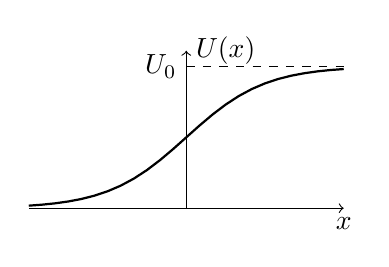
\begin{tikzpicture}
	\draw[->] (-2,0)--(2,0);
	\draw[->] (0,0)--(0,2);
	\draw[dashed] (0,1.8)--(2,1.8);
	\draw[ thick,domain =-2:2] plot(\x,{1.8/(1+exp(-2*\x)))});
	\coordinate[label=right:$ U(x) $](Ux) at (0,2);
	\coordinate[label=below:$ x $](x) at (2,0);
	\coordinate[label=left:$ U_0 $](U0) at (0,1.8);
	\end{tikzpicture}\caption{FIG. 5}\label{Fig.5}
\end{wrapfigure}
phenomenon appears: even for $ E > U_0 $, the particle may be reflected from the potential wall. The probability of reflection must in principle be calculated as follows.




Let the particle be moving from left to right. For large positive values of $ x $, the wave function must describe a particle which has passed “above the wall” and is moving in the positive direction of $ x $, i.e. it must have the asymptotic form
\begin{equation}\label{25.1}
\text{for }x\to\infty\colon\quad\psi\approx A\e^{\i k_2 x},\quad k_2=\frac{1}{\h}\sqrt{2m(E-U_0)}
\end{equation}
and $ A $ is a constant. To find the solution of Schr\"odinger's equation which satisfies this boundary condition, we calculate the asymptotic expression for $ x \to-\infty $; it is a linear combination of the two solutions of the equation of free motion, i.e. it has the form
\begin{equation}\label{25.2}
\text{for }x\to-\infty\colon\quad\psi\approx \e^{\i k_1 x}+B\e^{-k_1 x},\quad k_1=\frac{1}{\h}\sqrt{2mE}.
\end{equation}


The first term corresponds to a particle incident on the wall (we suppose $\psi$ normalized so that the coefficient of this term is unity); the second term represents a particle reflected from the wall. The probability current density in the incident wave is $ k_1 $, in the reflected wave $ k_1|B|^2 $, and in the transmitted wave $ k_2|A|^2 $. We define the \textit{transmission coefficient} $ D $ of the particle as the ratio of the probability current density in the transmitted wave to that in the incident wave:
\begin{equation}\label{25.3}
D=\frac{k_2}{k_1}|A|^2.
\end{equation}
Similarly we can define the reflection coefficient $ R $ as the ratio of the density in the reflected wave to that in the incident wave. Evidently $ R = 1 − D $:
\begin{equation}\label{25.4}
R=|B|^2=1-\frac{k_2}{k_1}|A|^2
\end{equation}
(this relation between $ A $ and $ B $ is automatically satisfied).

If the particle moves from left to right with energy $ E < U_0 $, then $ k_2 $ is purely imaginary, and the wave function decreases exponentially as $ x \to+\infty $. The reflected current is equal to the incident one, i.e. we have “total reflection” of the particle from the potential wall. We emphasize, however, that in this case the probability of finding the particle in the region where $ E < U $ is still different from zero, though it diminishes rapidly as $ x $ increases.

In the general case of an arbitrary stationary state (with energy $ E > U_0 $), the asymptotic form of the wave function is given, both for $ x \to-\infty $ and for $ x \to+\infty $, by a sum of waves propagated in each direction:
\begin{equation}\label{25.5}
\begin{split}
\psi&=A_1\e^{\i k_1x}+B_1\e^{-\i k_1x}\quad\text{for}\quad x\to-\infty,\\
\psi&=A_2\e^{\i k_2x}+B_2\e^{-\i k_2x}\quad\text{for}\quad x\to+\infty.
\end{split}
\end{equation}
Since these expressions are asymptotic forms of the same solution of a linear differential equation, there must be a linear relation between the coefficients $ A_1 $, $ B_1 $ and $ A_2 $, $ B_2 $. Let $ A_2 =\alpha A_1 + \beta B_1 $, where $\alpha$, $\beta$ are constants (in general complex) which depend on the specific form of the field $ U (x) $. The corresponding relation for $ B_2 $ can then be written down from the fact that Schr\"odinger's equation is real. This shows that, if $\psi$ is a solution of a given Schr\"odinger's equation, the complex conjugate function $\psi^*$ is also a solution. The asymptotic forms
\begin{equation*}
\begin{split}
\psi^*&=A_1^*\e^{-\i k_1x}+B_1^*\e^{\i k_1x}\quad\text{for}\quad x\to-\infty,\\
\psi^*&=A_2^*\e^{-\i k_2x}+B_2^*\e^{\i k_2x}\quad\text{for}\quad x\to+\infty
\end{split}
\end{equation*}
differ from \eqref{25.5} only in the nomenclature of the constant coefficients; we therefore have $ B_2^* = \alpha B_1^* + \beta A_1^* $ or $ B2 = \alpha^*B_1 + \beta^*A_1 $. Thus the coefficients in \eqref{25.5} are related by equations of the form
\begin{equation}\label{25.6}
A_2=\alpha A_1+\beta B_1,\quad B_2=\beta^*A_1+\alpha^*B_1.
\end{equation}


The condition of constant current along the $ x $-axis leads to the relation
\[ k_1(|A_1|^2-|B_1|^2)=k_2(|A_2|^2-|B_2|^2). \]
Expressing $ A_2 $, $ B_2 $ in terms of $ A_1 $, $ B_1 $ by \eqref{25.6}, we find
\begin{equation}\label{25.7}
|\alpha|^2-|\beta|^2=\frac{k_1}{k_2}.
\end{equation}


Using the relation \eqref{25.6}, we can show, in particular, that the reflection coefficients are equal (for a given energy $ E > U_0 $) for particles moving in the positive and negative directions of the $ x $-axis; the former case corresponds to putting $ B_2 = 0 $ in \eqref{25.5}, and the latter case to $ A_1 = 0 $. In these two cases, $ B_1/A_1 = −\beta^*/\alpha^* $ and $ A_2/B_2 = \beta/\alpha^* $ respectively. The corresponding reflection coefficients are
\[ R_1=\left|\frac{B_1}{A_1} \right|^2=\left|\frac{\beta^*}{\alpha^*}\right|^2,\quad R_2=\left|\frac{A_2}{B_2}\right|^2=\left|\frac{\beta}{\alpha^*}\right|^2 \]
whence it is clear that $ R_1 = R_2 $.

It is natural to call $ B_1/A_1 = -\beta^*/\alpha^* $ and $ A_2/B_2 = \beta/\alpha^* $ the \textit{reflection amplitudes} for motion in the positive and negative directions respectively. They are equal in modulus but may have different phase factors.





{\small
\textbf{PROBLEMS}


\textbf{1.} Determine the reflection coefficient of a particle from a rectangular potential wall (Fig. \ref{Fig.6}); the energy of the particle $ E > U_0 $.


\begin{wrapfigure}[]{l}[0cm]{0cm}
	\begin{tikzpicture}
	\draw[->] (-1,0)--(2.5,0);
	\draw[->] (0,0)--(0,2);
	\draw[thick] (-1,0)--(0,0)--(0,1.5)--(2,1.5);
	\coordinate[label=right:$ U(x) $](Ux) at (0,2);
	\coordinate[label=right:$ x $](x) at (2.5,0);
	\coordinate[label=left:$ U_0 $](U0) at (0,1.5);
	\end{tikzpicture}\caption{FIG. 6}\label{Fig.6}
\end{wrapfigure}






SOLUTION. Throughout the region $ x > 0 $, the wave function has the form \eqref{25.1}, while in the region $ x < 0 $ its form is \eqref{25.2}. The constants $ A $ and $ B $ are determined from the condition that $\psi$ and $\d\psi/\d x $ are continuous at $ x = 0 $:
\[ 1+B=A,\quad k_1(1-B)=k_2 A, \]
whence
\[ A=\frac{2k_1}{k_1+k_2},\quad B=\frac{k_1-k_2}{k_1+k_2}. \]
The reflection coefficient\footnote{In the limiting case of classical mechanics, the reflection coefficient must become zero. The expression obtained here, however, does not contain the quantum constant at all. This apparent contradiction is explained as follows. The classical limiting case is that in which the de Broglie wavelength of the particle $ \lambda\sim\h/p $ is small in comparison with the characteristic dimensions of the problem, i.e. the distances over which the field $ U (x) $ changes noticeably. In the schematic example considered, however, this distance is zero (at the point $ x = 0 $), so that the passage to the limit cannot be effected.} is \eqref{25.4}
\[ R=\left(\frac{k_1-k_2}{k_1+k_2} \right)^2\left(\frac{p_1-p_2}{p_1+p_2} \right)^2 \]
For $ E = U_0 $ ($ k_2 = 0 $), $ R $ becomes unity, while for $ E \to\infty $ it tends to zero as $ R=(U_0/4E)^2 $.





\textbf{2.} Determine the transmission coefficient for a rectangular potential barrier (Fig. \ref{Fig.7}).










SOLUTION. Let $ E $ be greater than $ U_0 $, and suppose that the incident particle is moving from left to right. Then we have for the wave function in the different regions expressions of the form
\begin{align*}
\psi&=\e^{\i k_1x}+A\e^{-\i k_1x}&\text{for }x&<0,\\
\psi&=B\e^{\i k_2 x}+B'\e^{-\i k_2x}&\text{for }0&<x<a,\\
\psi&=C\e^{\i k_1x}&\text{for }x&>a.
\end{align*}
(on the side $ x > a $ there can be only the transmitted wave, propagated in the positive direction of $ x $). The constants $ A $, $ B $, $ B' $ and $ C $ are determined from the
\begin{wrapfigure}[9]{r}[0cm]{0cm}
	\begin{tikzpicture}
	\draw[->] (-1.5,0)--(3,0);
	\draw[->] (0,0)--(0,2);
	\draw[thick] (-1.5,0)--(0,0)--(0,1.5)--(1.5,1.5)--(1.5,0)--(3,0);
	\coordinate[label=right:$ U(x) $](Ux) at (0,2);
	\coordinate[label=below:$ a $](a) at (1.5,0);
	\coordinate[label=left:$ U_0 $](U0) at (0,1.5);
	\end{tikzpicture}\caption{FIG. 7}\label{Fig.7}
\end{wrapfigure}
conditions of continuity of $\psi$ and $ \d\psi/\d x $ at the points $ x = 0 $ and $ a $. The transmission coefficient is determined as $ D = k_1|C|^2/k_1 = |C|^2 $. On calculating this, we obtain
\[ D=\frac{4k_1^2k_2^2}{(k_1^2-k_2^2)^2\sin^2ak_2+4k_1^2k_2^2} \]



For $ E < U_0 $, $ k_2 $ is a purely imaginary quantity; the corresponding expression for $ D $ is obtained by replacing $ k_2 $ by $ \i\varkappa_2 $ where $ \h\varkappa_2=\sqrt{2m(U_0-E)} $:
\[ D=\frac{4k_1^2\varkappa_2^2}{(k_1^2-\varkappa_2^2)^2\sin^2a\varkappa_2+4k_1^2\varkappa_2^2} \]




\textbf{3.} Determine the reflection coefficient for a potential wall defined by the formula 
\[ U (x) = U_0/(1 +\e^{-\alpha x}) \]
(Fig. \ref{Fig.5}); the energy of the particle is $ E > U_0 $.





SOLUTION. Schr\"odinger's equation is
\[ \frac{\d^2\psi}{{\d x}^2}+\frac{2m}{\h^2}\left(E-\frac{U_0}{1+\e^{-\alpha x}} \right)\psi=0. \]
We have to find a solution which, as $ x \to +\infty $, has the form
\[ \psi=\mathrm{const}\cdot\e^{\i k_2}. \]
We introduce a new variable
\[ \xi=-\e^{-\alpha x} .\]
(which takes values from $ -\infty $ to $ 0 $), and seek a solution of the form
\[ \psi=\xi^{-\i k_2/\alpha}w(\xi), \]
where $ w (\xi) $ tends to a constant as $ \xi\to 0 $ (i.e. as $ x \to\infty $). For $ w (\xi) $ we find an equation of hypergeometric type:
\[ \xi(1-\xi)w''+\left(1-\frac{2\i}{\alpha}k_2 \right)(1-\xi)w'+\frac{1}{\alpha^2}(k_2^2-k_1^2)w=0, \]
which has as its solution the hypergeometric function
\[ w=F\left[\frac{\i}{\alpha}(k_1-k_2),-\frac{\i}{\alpha}(k_1+k_2),-\frac{2\i}{\alpha}k_2+1,\xi \right] \]
(we omit a constant factor). As $ \xi\to0 $, this function tends to 1, i.e. it satisfies the condition imposed.

The asymptotic form of the function $\psi$ as $ \xi\to-\infty $ (i.e. $ x \to-\infty $) is\footnote{See formula (e.6), in each of whose two terms we must take only the first term of the expansion, i.e. replace the hypergeometric functions of $ 1/z $ by unity.
}
\begin{multline*}
\psi\approx\xi^{-\i k_2/\alpha}\left[C_1(-\xi)^{\i(k_2-k_1)/\alpha}+C_2(-\xi)^{\i(k_1+k_2)/\alpha} \right]=\\
=(-1)^{\i k_2/\alpha}\left[C_1\e^{\i k_1 x}+C_2^{-\i k_2 x} \right],
\end{multline*}
where
\begin{align*}
C_1&=\frac{\Gamma(-(2\i/\alpha)k_1)\Gamma(-(2\i/\alpha)k_2+1)}{\Gamma(-(\i/\alpha)(k_1+k_2))\Gamma(-(\i/\alpha)(k_1+k_2)+1)},\\
C_2&=\frac{\Gamma((2\i/\alpha)k_1)\Gamma(-(2\i/\alpha)k_2+1)}{\Gamma((\i/\alpha)(k_1-k_2))\Gamma((\i/\alpha)(k_1-k_2)+1)}.
\end{align*}
The required reflection coefficient is $ R = |C_2/C_1|^2 $ on calculating it by means of the well known formula
\[ \Gamma(x)\Gamma(1-x)=\frac{\pi}{\sin\pi x}, \]
we have
\[ R=\left\{\frac{\sinh\left[(\pi/\alpha)(k_1-k_2) \right]}{\sinh[(\pi/\alpha)(k_1+k_2)]} \right\}^2. \]
For $ E = U_0 $ ($ k_2 = 0 $), $ R $ becomes unity, while for $ E\to\infty $ it tends to zero as
\[ R=\left(\frac{\pi U_0}{\alpha\h} \right)^2\frac{2m}{E}\exp\left(-\frac{4\pi}{\alpha\h}\sqrt{2mE} \right). \]
In the limiting case of classical mechanics. $ R $ becomes zero, as it should.


\begin{wrapfigure}[6]{l}[0cm]{0cm}
	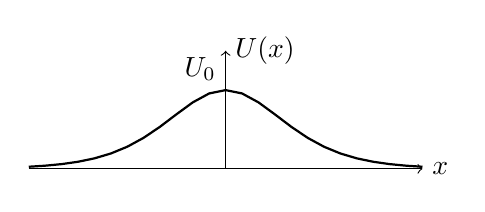
\begin{tikzpicture}
	\draw[->] (-2.5,0)--(2.5,0);
	\draw[->] (0,0)--(0,1.5);
	\draw[ thick,domain =-2.5:2.5] plot(\x,{1/(cosh(\x)*cosh(\x))))});
	\coordinate[label=right:$ U(x) $](Ux) at (0,1.5);
	\coordinate[label=right:$ x $](x) at (2.5,0);
	\coordinate[label=above left:$ U_0 $](U0) at (0,1);
	\end{tikzpicture}\caption{FIG. 8}\label{Fig.8}
\end{wrapfigure}




\textbf{4.} Determine the transmission coefficient for a potential barrier defined by the formula
\[ U(x)=\frac{U_0}{\cosh^2\alpha x} \]
(Fig. \ref{Fig.8}); the energy of the particle is $ E < U_0 $.






SOLUTION. The Schr\"odinger's equation is the same as that obtained in the solution of Problem 5, \S\ref{The linear oscillator}; it is necessary merely to alter the sign of $ U_0 $ and to regard the energy $ E $ now as positive. A similar calculation gives the solution
\begin{equation}\label{25-1}
\psi=(1-\xi^2)^{-\frac{\i k}{2\alpha}}F\left(-\frac{\i k}{\alpha}-s,-\frac{\i k}{\alpha}+s+1,-\frac{\i k}{\alpha}+1,\frac{1-\xi}{2} \right),\tag{1}
\end{equation}
where
\[ \xi=\tanh\alpha x,\quad k=\frac{1}{\h}\sqrt{2mE},\quad s=\frac{1}{2}\left(-1+\sqrt{1-\frac{8mU_0}{\alpha^2\h^2}} \right). \]
This solution satisfies the condition that, as $ x \to\infty $ (i.e. as $ \xi\to1$, $(1-\xi)\approx2\e^{-2\alpha x} $ ), the wave function should include only the transmitted wave ($ \sim\e^{\i kx} $). The asymptotic form of the wave function as $ x\to-\infty (\xi\to−1) $ is found by transforming the hypergeometric function with the aid of formula (e.7):
\begin{equation}\label{25-2}
\psi\sim\e^{\i kx}\frac{\Gamma(\i k/\alpha)\Gamma(1-\i k/\alpha)}{\Gamma(-s)\Gamma(1+s)}+\e^{\i kx}\frac{\Gamma(-\i k/\alpha)\Gamma(1-\i k/\alpha)}{\Gamma(-\i k/\alpha-s)\Gamma(-\i k/\alpha+s+1)}.\tag{2}
\end{equation}
Taking the squared modulus of the ratio of coefficients in this function, we obtain the following expression for the transmission coefficient $ D = 1 − R $:
\begin{align*}
D&=\frac{\sinh^2\frac{\pi k}{\alpha}}{\sinh^2\frac{\pi k}{\alpha}+\cos^2\left(\frac{\pi}{2}\sqrt{1-\frac{8mU_0}{\h^2\alpha^2}} \right)}\qquad\text{if}\quad\frac{8mU_0}{\h^2\alpha^2}<1,\\
D&=\frac{\sinh^2\frac{\pi k}{\alpha}}{\sinh^2\frac{\pi k}{\alpha}+\cosh^2\left(\frac{\pi}{2}\sqrt{\frac{8mU_0}{\h^2\alpha^2}-1} \right)}\qquad\text{if}\quad\frac{8mU_0}{\h^2\alpha^2}>1.
\end{align*}
The first of these formulae holds also for the case $ U_0 < 0 $, i.e. when the particle is passing over a potential well instead of a potential barrier. It is interesting to note that in that case $ D = 1 $ if $ 1 +8m|U_0|/\h^2\alpha^2 = (2n + 1)^2 $; thus, for certain values of the depth $ |U_0| $ of the well, particles passing over it are not reflected. This is evident from equation \eqref{25-2}, where the term in $ \e^{\i kx} $ vanishes for positive integral $ s $.





\textbf{5.} Determine how the transmission coefficient tends to zero as $ E \to0 $, assuming that the potential energy $ U (x) $ decreases rapidly at distances $ |x|\gg a $, where $ a $ is the dimension of the interaction region.





SOLUTION. For distances $ k |x| \ll1 $, $ E $ can be neglected in Schr\"odinger's equation. If also $ |x|\gg a $, the potential energy can also be neglected, and the equation becomes
\[ -\frac{\h^2}{2m}\frac{\d^2\psi}{{\d x}^2}=0, \]
the solution of this may be written as
\begin{equation}\label{25-3}
\psi=a_1+b_1x,\quad x<0,\qquad\psi=a_2+b_2x,\quad x>0.\tag{1}
\end{equation}

The relation between $ a_1 $, $ b_1 $ and $ a_2 $, $ b_2 $ can be found by solving the equation at distances $ |x|\sim a $. It is linear:
\begin{equation}\label{25-4}
a_1=\rho a_2+\mu b_2,\quad b_1=\nu a_1+\tau b_2.\tag{2}
\end{equation}
The coefficients $ \rho $, $ \mu $, $ \nu $ and $ \tau $ are real and independent of the energy, which does not appear in the equation.\footnote{Since the flux is constant, $ \rho\tau-\mu\nu= 1 $.
} The solution \eqref{25-3} must be the same as the first two terms in the expansion of \eqref{25.1} and \eqref{25.2} in powers of $ x $, so that
\[a_1=B+1,\quad b_1=\i k(1-B),\quad a_2=A,\quad b_2=\i kA. \]
Substituting these in \eqref{25-4} and solving for $ A $, we get, for small $ k\colon A \approx2\i k/\nu $, whence 
\[ D\approx\frac{4k^2}{\nu^2}\sim E \]
The transmission coefficient thus tends to zero in proportion to the particle energy. This is of course true for the examples in Problems 2 and 4.}